\documentclass[conf]{new-aiaa}
%\documentclass[journal]{new-aiaa} for journal papers
\usepackage[utf8]{inputenc}

\usepackage{graphicx}
\usepackage{float}
\usepackage{amsmath}
\usepackage[version=4]{mhchem}
\usepackage{siunitx}
\usepackage{longtable,tabularx}
\usepackage[version=4]{mhchem}
\usepackage{subcaption}
\setlength\LTleft{0pt} 
\usepackage{amsmath}
\usepackage{amssymb}
\usepackage{natbib}
\usepackage{bm}
\renewcommand{\vec}[1]{\mathbf{#1}}
\usepackage[T1]{fontenc}
\usepackage[framed,numbered]{matlab-prettifier}
\lstset{
	style = Matlab-editor,
	basicstyle=\mlttfamily\small,
}



\title{\pmb{\mathcal{$N$}}-Body Simulations to Solve Planetary Systems and Arenstorf Translunar Insertions}

\author{Parthiv Kukadia}\affil{Aerospace Engineering, University of Illinois at Urbana Champaign}

\begin{document}

\maketitle

\begin{abstract}
This paper describes the implementation and analysis of the Forward Euler (FE), Heun, Kick-Drift-Kick (KDK), and RK4 numerical methods to simulate various $\mathcal{$N$}$-body problems with the goal of being able to solve for Arenstorf orbits to enable a Translunar Insertion (TLI). After analyzing the stability regions of these numerical methods, examining the effect that time step size and truncation error have on various simulations, and validating their accuracy by comparing their results to real planetary orbit data from JPL, the stable TLI used by the Apollo missions was solved for and replicated accurately.
\end{abstract}

\section{Nomenclature}

{\renewcommand\arraystretch{1.0}
\noindent\begin{longtable*}{@{}l @{\quad=\quad} l@{}}
$G$  & universal gravitation constant (6.674 \times $ 10^{-11}$ N\cdot \text{m} $^2$/kg$^2$) \\
$x_i, y_i, z_i$ & Cartesian coordinate components of the $i^{th}$ body (m) \\
$x^*, y^*, z^*$ & synodic coordinate components of the $i^{th}$ body (m) \\
$N$ & number of bodies in an $N-Body$ simulation\\
$r_j$ &  distance from the $j^{th}$ orbital body to the origin of the reference frame (m) \\
$r_true$, $\dot{r}_true$ & true position and velocity of a body obtained from JPL data (m) (m/s)\\
$\dot{r}_j$, $\ddot{r}_j$ & velocity and acceleration of the $j^{th}$ orbital body (m/s) (m/s$^2$)\\
$m_j$& mass of the $j^{th}$ orbital body (kg) \\
$M$ & total mass of an $N$-body system (kg)\\
$\alpha$ & ratio between the mass of the $N=1$ body and the total system mass\\
$\mu$  & ratio between the mass of the $N=2$ body and the total system mass \\
$D$ & length of the semi-major axis of an $N=2$ system (m)\\
$t$ & point in time (s)\\
$\Delta t$ & time step (s) \\
$T_j$ & orbital period of the $j^{th}$ body (s)\\
$n$ & number of orbital periods\\
$\omega$ & angular velocity of an orbital body (rad/s)  \\
$\lambda$ & complex numbered eigenvalues\\
\end{longtable*}}

\section{Introduction}
The $N$-body problem aims to simulate and predict planetary motion for $N$ orbital bodies that exert gravitational forces on each other. Even though solutions cannot be found analytically for $N>2$, numerical methods offer various solutions to solving $N$-body problems for a variety of $N$ with different initial conditions and configurations \cite{britt}. For a system of $N$ bodies
\begin{align}
	\bm{r}_j &= \begin{bmatrix}
		(r_x)_j \\ (r_y)_j \\ (r_z)_j
	\end{bmatrix}, \quad j = 1, \dots, N
&
	\bm{\dot{r}}_j &= \begin{bmatrix}
		(\dot{r}_x)_j \\ (\dot{r}_y)_j \\ (\dot{r}_z)_j
	\end{bmatrix}, \quad j = 1, \dots, N
\end{align} 
can be used to initialize and represent the positions and velocities of all bodies in space at any given time. To account for the gravitational impact of the orbital bodies on each other, Newton's Law of Gravitation can be used, such that

\begin{equation}
	\bm{\ddot{r}}_i = \bm{\dot{v}}_i = \sum_{\substack{j=1 \\ j \ne i}} ^{N} \frac{G m_j (\bm{r}_j-\bm{r}_i)}{||\bm{r}_j-\bm{r}_i||^3} \label{rddot}	
\end{equation}
where $\ddot{r_i}$ is acceleration of the $i^{th}$ orbital body and $G$ is the gravitational constant. Using this equation of motion and the initialized conditions, the $N$-body system is now in a form that can be represented by the chosen numerical methods.
\section{Overview}
    \subsection{Numerical Methods}
    The numerical methods that were utilized to solve the N-body problem were Forward Euler, Heun's method, RK4, and Kick-Drift-Kick \cite{LecOSM}. These various methods were implemented to allow a comparison in the accuracy of these methods for the N-body problem \cite{Bill}. To implement different numerical methods, it is important to define an initial value problem in the form shown below:
    \begin{equation}
        \bm{\dot{u}} = \bm{f(u},t)
        \label{udot}
    \end{equation}
    \begin{equation}
        \bm{u}(t_{0}) = \bm{u}_{0}
        \label{ui}
    \end{equation}
    The equation provided in \eqref{rddot} allows the placement of the N-body equation in the form that is required to solve an initial value problem given in \eqref{udot} and \eqref{ui}. This helps in creating a column vector, $\boldsymbol{u}$, which contains both position and velocity, shown as a stack vector:
    \begin{equation}
        \boldsymbol{u} = \begin{bmatrix}
        \bm{r}_1 & \bm{v}_1 & \hdots & \bm{r}_2 & \bm{v}_2 & \hdots & \bm{r}_N & \bm{v}_N
        \end{bmatrix}^T
        \label{u}
    \end{equation}
    Which helps in rewriting the initial condition as the following:
    \begin{equation}
        \boldsymbol{u}(t_0) = \begin{bmatrix}
        \bm{r}_1(t_0) & \bm{v}_1(t_0) & \hdots & \bm{r}_2(t_0) & \bm{v}_2(t_0)  & \hdots & \bm{r}_N(t_0) & \bm{v}_N(t_0)
        \end{bmatrix}^T
        \label{u}
    \end{equation}
    Therefore, $\bm{\dot{u}}$ can be expressed as shown below:
    \begin{equation}
        \bm{\dot{u}} = \begin{bmatrix}
        \bm{\dot{r}}_1 & \bm{\dot{v}}_1 & \hdots & \bm{\dot{r}}_2 & \bm{\dot{v}}_2  & \hdots & \bm{\dot{r}}_N& \bm{\dot{v}}_N
        \end{bmatrix}^T
    \end{equation}
    Therefore, it is shown that the second order differential equation \eqref{rddot} has successfully been expressed as a first order differential equation, allowing the application of the various different numerical methods to solve for positions and velocities for the N-body problem that will be explored. 
        \subsubsection{Forward Euler}
        Forward Euler is one the one-step methods used to derive a finite difference for IVP. In fact, it is known to be the simplest finite difference. Forward Euler is a function formed to be explicit, where the following is obtained \cite{LecOSM}: 
        \begin{equation}
            u_{i+1} = u_{i} + {\Delta t}f(u_{i})
        \end{equation}
        
        \subsubsection{Heun's Method}
        Heun's Method is also known as the second-order Runge-Kutta method. It can be derived by restricting the multi-stage methods from the Trapezoid Method. Using Taylor series to numerically derive Heun's Method, the following is obtained \cite{LecOSM}: 
        \begin{equation}
            u_{i+1} = u_{i} + \frac{\Delta t}{2}[f(u_{i})+f(u_i+{\Delta t}f(u_{i}))]
        \end{equation}
        where it can be written as:
        \begin{equation}
            \bm{u}_{i+1} = u_i + \frac{1}{4}k_1 + \frac{3}{4}k_2
        \end{equation}
        in which,
        \begin{equation*}
            k_1 = \Delta t f(u_i,t_i) 
        \end{equation*}
        \begin{equation*}
             k_2 = \Delta t f(u_i + \frac{2}{3}k_1 , t_i + \frac{2}{3}\Delta t)
        \end{equation*}
        \subsubsection{RK4}
        RK4 is the fourth-order Runge-Kutta method. When numerically integrating a RK4 scheme, the following formula is obtained \cite{LecOSM}:
        \begin{equation}
            u_{i+1} = u_{i} + \frac{\Delta t}{6}(k_1 + 2k_2 + 2k_3 + k_4)
        \end{equation}
        in which:
        \begin{equation*}
            k_1 = f(u_i,t_i)
        \end{equation*}
        \begin{equation*}
            k_2 = f(u_i + \frac{1}{2}\Delta t k_1 , t_i + \frac{1}{2} \Delta t)
        \end{equation*}
        \begin{equation*}
            k_3 = f(u_i + \frac{1}{2}\Delta t k_2, t_i + \frac{1}{2} \Delta t)
        \end{equation*}
        \begin{equation*}
            k_4 = f(u_i + \Delta t k_3 , t_i + \Delta t)
        \end{equation*}
        
        \subsubsection{KDK}
        KDK is a form of a leapfrog method, also known as, "Kick-Drift-Kick"\cite{NumMeth}. This method is considered to be beyond the scope of the numerical methods course because it is a unique, interesting concept not taught yet. In order to establish a 2nd-order of accuracy, it is required to take half-steps when computing a particle's position. Numerically integrating the KDK method, the following is obtained\cite{StabLF}: 
        \begin{equation}
            r_{i+\frac{1}{2}} = r_{i} + v_{i}\frac{\Delta t}{2} 
        \end{equation}
        \begin{equation}
            v_{i+1} = v_{i} + f(r_{i+\frac{1}{2}})\Delta t
        \end{equation}
        \begin{equation}
            r_{i+1} = r_{i+\frac{1}{2}} + v_{i+1}\frac{\Delta t}{2} 
        \end{equation}
        This numerical method was used because of it's second order accuracy. KDK is also non-dissipative, which means that the numerical method does not have any thermodynamically irreversible transformation of potential or kinetic energy into any other forms of energy that could potentially be decrease the systems ability to perform work. KDK also only requires one function evaluation per $\Delta t$. However, there are some downsides for using KDK, considering it's absolute stability region is on an interval that is only located on the imaginary axis $I(\lambda_{i} \Delta t)$ which will be derived below \cite{LeapFTI}.
    \subsection{Global Truncation Error}
    Truncation error is the error associated in the evaluation of $\bm{\dot{u}}$, to provide the accuracy of the numerical methods that were implemented. Truncation error shows the error relating the advancement of the method from an initial time-step to the following one and so on. Truncation error can be obtained by substituting the exact solution into the numerical method, followed by dividing by the time step, $\Delta t$ \cite{LecER}.
        \subsubsection{Forward Euler}
        Looking at the truncation error derivation associated with forward Euler, the following is obtained \cite{LecER}:
        \begin{equation}
            \tau_i = \frac{\bm{u}(t_{i+1}) - \bm{u}(t_i)}{\Delta t} - \bm{f}(\bm{u}(t_i),t_i) \label{FET}
        \end{equation}
        The truncation error associated with using forward Euler method is as follows:
        \begin{equation}
            \bm{\tau_i} = O(\Delta t) \label{FETrunc}
        \end{equation}
        Solving \eqref{FET} using Taylor series, the following derivations are obtained \cite{LecER}:
        \begin{equation}
        \begin{aligned}
        &\bm{\tau}_{i}=\frac{\bm{u}\left(t_{i+1}\right)-\bm{u}\left(t_{i}\right)}{\Delta t}-\bm{f}\left(\bm{u}\left(t_{i}\right), t_{i}\right)\\
        & =\frac{\bm{u}\left(t_{i+1}\right)-\bm{u}\left(t_{i}\right)}{\Delta t}-\dot{\bm{u}}\left(t_{i}\right) \\
        &=\frac{\bm{u}\left(t_{i+1}\right)-\bm{u}\left(t_{i}\right)}{\Delta t}-\frac{\bm{u}\left(t_{i+1}\right)-\bm{u}\left(t_{i}\right)}{\Delta t}+\mathrm{O}(\Delta t)\\
        &\therefore \quad \bm{\tau}_{i}=O(\Delta t) \label{FOREULT}
        \end{aligned}
        \end{equation}
        In the derivation shown above in \eqref{FOREULT}, line 2 implements the definition of an Initial Value Problem, and to obtain the results in line 4, a Taylor Series expansion is done in line 3 of $\bm{u}(t_i)$ about $t_{i+1}$ \cite{LecER}. As shown in the derivation above, the truncation error associated with forward Euler can be written as shown in \eqref{FETrunc}.
        
        \subsubsection{Heun's Method}
        One step methods all have identical processes to derive the truncation error\cite{LecER}. Therefore using the same steps that were used in \eqref{FOREULT}, the truncation error for Heun's method can be derived to the following:
        \begin{equation}
            \tau_i = O(\Delta t^2)
        \end{equation}
        The following Taylor series expansion is obtained once the steps done in \eqref{FOREULT} are conducted for $\bm{u}(t_i)$ about $t_{i+1}$, resulting in:
        \begin{equation}
        \bm{u}(t_i) = \bm{u}(t_{i+1}) + \Delta t\bm{\dot{u}}(t_{i+1})+ H.O.T. \label{TruncH}
        \end{equation}
        It is used in helping derive the truncation error for Heun's method, which turns out to be $\tau_i = O(\Delta t^2)$ as shown above.
        
        \subsubsection{RK4}
        Looking at the RK4 truncation derivation, the following is obtained\cite{LecER}:
        \begin{equation}
            \tau_i = \frac{\bm{u}(t_{i+1}) - \bm{u}(t_i)}{\Delta t} - \frac{1}{6}(\bm{y}_1 + 2\bm{y}_2 + 2\bm{y}_3 + \bm{y}_4) \label{tau}
        \end{equation}
    Equation \eqref{tau} shown above can be represented in the form of the initial value problem \eqref{udot}. The representation of \eqref{tau} in the form of an IVP can then help derive the truncation error through the use of Taylor series. The truncation error that should be obtained for RK4 can be written as:
    \begin{equation}
        \tau_k = O(\Delta t^4) \label{TRK4}
    \end{equation}
    The steps conducted in \eqref{FOREULT} are the same steps that were conducted to derive the truncation error associated with RK4, however they were not implemented in the report due to the similarity of the derivation shown for forward Euler. The following Taylor series expansion is obtained once those steps are conducted for $\bm{u}(t_i)$ about $t_{i+1}$\cite{LecER}:
    \begin{equation}
        \bm{u}(t_i) = \bm{u}(t_{i+1}) + \Delta t\bm{\dot{u}}(t_{i+1}) + \frac{\Delta t^2}{2}\bm{\ddot{u}}(t_{i+1}) + \frac{\Delta t^3}{6}\bm{\dddot{u}}(t_{i+1}) + H.O.T. \label{TruncRK4}
    \end{equation}
    Thus, this expansion allows equation \eqref{TRK4} to be obtained, showing the truncation error for RK4 being derived successfully. 
    \subsubsection{KDK}
    KDK, also known as midpoint, being a 2nd order scheme like Huen's method also has a truncation error of:
    \begin{equation}
        \tau_i= O(\Delta t^2)
    \end{equation}
    The method can be computed by placing the model in the form \cite{TruncErrLF}:
    \begin{equation}
        \bm{u}_{i+1} = \bm{u}_{i-1} + 2\Delta t \bm{u}(t_i,\bm{u}_i) \label{KDKModel}
    \end{equation}
    Thus, it can be derived from computing a difference scheme using Taylor series\cite{TruncErrLF}:
    \begin{equation}
        \bm{u}(t_i + \Delta t) = u(t_i) + \Delta t \bm{\dot{u}}(t_i,u(t_i)) + \frac{\Delta t^2}{2}\bm{\ddot{u}}(t_i,u(t_i)) + \frac{\Delta t^3}{6}\bm{\dddot{u}}(t_i,u(t_i)) + H.O.T
    \end{equation}
    \begin{equation}
        \bm{u}(t_i - \Delta t) = u(t_i) - \Delta t \bm{\dot{u}}(t_i,u(t_i)) + \frac{\Delta t^2}{2}\bm{\ddot{u}}(t_i,u(t_i)) - \frac{\Delta t^3}{6}\bm{\dddot{u}}(t_i,u(t_i)) + H.O.T
    \end{equation}
    Substituting the equations derived above into the leapfrog scheme shown in equation \eqref{KDKModel}, the following is obtained\cite{TruncErrLF}:
    \begin{equation}
        \bm{u}(t_i + \Delta t) = \bm{u}(t_i - \Delta t) + 2\Delta t \bm{u}(t_i,\bm{u}(t_i)) + O(\Delta t^3)
    \end{equation}
    Which results in a global truncation error of $\tau_i = O(\Delta t^2)$. This result matches the theoretical result obtained conceptually regarding the global error of a 2nd order method.
    
    \subsection{Stability}
    This section will go over the regions of stability present for the different numerical methods that have been explored. Stability is important in understanding whether or not the accuracy of a numerical method was determined correctly\cite{NumSol}. The accuracy of a numerical method that has been implemented is determined through calculating the truncation error. However, this is only possible if the numerical method being implemented is stable \cite{UoV}. The reason stability is crucial in predicting the accuracy of a numerical method relies on the fact that the derivation of truncation error, which is obtained through taylor series is valid only for small $\Delta t$'s, and therefore, to obtain the dependence for larger $\Delta t$'s for a finite difference method, we must take into consideration stability \cite{LecAS}.
    A numerical method implementation to solve an initial value problem (IVP) is stable if small disturbances in the initial conditions of the problem don't result to divergence of the numerical approximations away from the true solutions, assuming that the IVP is bounded. A numerical method is absolutely stable if the numerical solution behaves in a controlled fashion. Applying this to the N-body problem means that the solution we obtain is stable if none of the bodies behave in a manner that cannot be controlled; the bodies remain in a consistent orbit without gravitating/diverging away from the system permanently \cite{DiffEq}.
    
    The figure shown below includes the different stability regions for the different numerical methods that were explored where the regions within the lines are the absolute stability regions\cite{StabReg}:
    \begin{figure}[H]
        \centering
        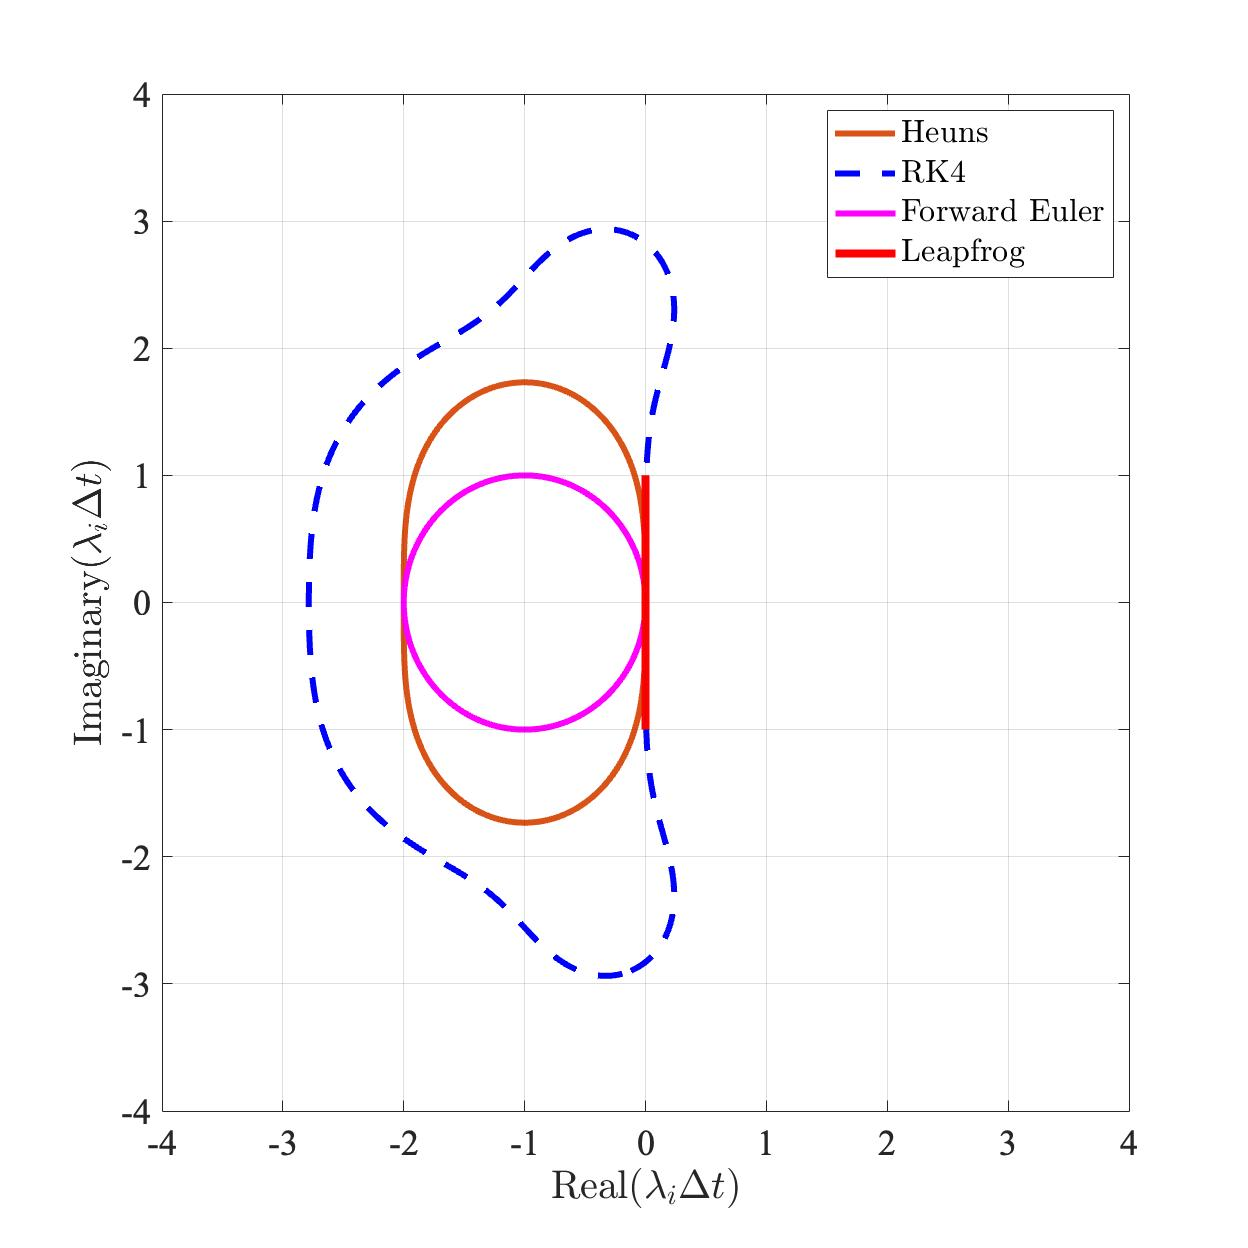
\includegraphics[height = 13cm]{Figures/Stability/Stability.jpg}
        \caption{Stability Regions for Various Numerical Methods}
        \label{Stab}
    \end{figure}
  
    To be able to determine the stability of a method, a model is required, such that\cite{LecAS}:
    \begin{equation}
        \bm{\dot{u}} = \bm{\Lambda u} \label{MIVP}
    \end{equation}
    \begin{equation}
        \bm{t}_0 = \bm{u}_0
    \end{equation}
    in which $\bm{\Lambda}$ is given as a diagonal matrix shown below:
    \begin{equation}
        \bm{\Lambda} = \begin{bmatrix}
        \lambda_1 & 0 & \hdots & 0 & 0\\
        0 & \lambda_2 & \hdots & 0 & 0\\
        \vdots & \vdots & \hdots & \vdots & \vdots\\
        0 & 0 & \hdots & \lambda_{n-1} & 0\\
        0 & 0 & \hdots & 0 & \lambda_n
        \end{bmatrix}
    \end{equation}
    where each $\lambda_l \in \mathbb{C}$, with $l = 1, \hdots,n$. Therefore, using the definition of $e^{\Lambda t}$, the exact solution's $j^{th}$ component is obtained through:
    \begin{equation}
        u_j(t) = e^{\lambda_j(t-t_0}(u_0)_j \label{ujt}
    \end{equation}
    In equation \eqref{ujt}, the term $(u_0)_j$ refers to the $j^{th}$ entry of $u_0$.
    Applying one-step methods such as Forward Euler, Heun's method and RK4 to the modelled IVP above, the absolute stability region for one-step methods is when for values of $\Delta t \lambda_{l}$ \cite{LecAS}
    \begin{equation}
        |R(z)| = |R(\Delta t \lambda_{l})| < 1 \label{GeneralizedStab}
    \end{equation}
    A method is unstable/chaotic when values of $\Delta t\lamda_{i}$ do not satisfy the requirement above. Therefore, to compute the absolute stability regions, only $R(z)$ is needed for the given one-step method, where you need to identify the different values of z for which the above requirement is fulfilled. Values of $\Delta t \lambda_l$ that fulfilled the requirements given through equation \eqref{GeneralizedStab}, and is also a stable region for the values that were chosen in this project for the various different numerical methods that were explored .
        \subsubsection{Forward Euler}
        Once the IVP has been modelled, different numerical methods can be applied to obtain the absolute stability regions. Applying forward Euler to the modelled IVP shown above, forward Euler can be expressed as\cite{LecAS}:
        \begin{equation}
        \begin{aligned}
        \bm{u}_{k+1} &=\bm{u}_{k}+\Delta t \bm{\Lambda} \bm{u}_{k} \\
        &=(\bm{I}+\Delta t \bm{\Lambda}) \bm{u}_{k} \\
        &=(\bm{I}+\Delta t \bm{\Lambda})(\bm{I}+\Delta t \bm{\Lambda}) \bm{u}_{k-1} \\
        &=(\bm{I}+\Delta t \bm{\Lambda})^{k+1} \bm{u}_{0}
        \end{aligned}
        \end{equation}
        thus, the $j^{th}$ component of the exact solution is given by:
        \begin{equation}
            (u_{k+1})_j = (1 + \Delta t \lambda_j)^{k+1}(u_0)_j
        \end{equation}
        Therefore, if $|1 + \Delta t\lamda_j| > 1$ the iterates of the IVP will grow without a bound as k tends to infinity. Keep in mind that $\lambda_{i}$ and $\Delta t$ are not important separately, but very important together, such that the forward Euler method is absolutely stable when: 
        \begin{equation}
            |R(z)| = |1 + \Delta t \lambda_{j}| < 1
        \end{equation}
        Thus the following condition is obtained for $\Delta t$, where:
        \begin{equation}
            \Delta t < \frac{2}{\lambda_j}
        \end{equation}
        If the above requirement is satisfied, a solution is obtained that is within the stability region shown above in figure \ref{Stab}.
        
        \subsubsection{Heun's Method}
        Therefore, using the modelled IVP shown in equation \eqref{MIVP}, and the exact solution's $j^{th}$ component shown in equation \eqref{ujt}, the Heun's method scheme can be expressed as\cite{StabH}:
        \begin{equation}
        (\bm{u}_{k+1})_j = \bm{u}_{k}\left(1 + \Delta t \lambda_j + \frac{1}{2}(\Delta t \lambda_j)^2\right)
        \end{equation}
        Thus, the boundary for the absolute stability region is given as:
        \begin{equation}
            |R(z)| = \left|1 + \Delta t \lambda_j + \frac{1}{2}(\Delta t \lambda_j)^2\right| < 1
        \end{equation}
        Wherein if the absolute value is equal to 1, the condition that needs to be satisfied can be written as:
       \begin{equation}
           \left(1+ \Delta t \lambda_j + \frac{1}{2}((\Delta t \lambda_R)^2 - (\Delta t \lambda_I)^2)\right)^2 + \left(\Delta t \lambda_I + \Delta t^2 \lambda_I\lambda_R\right)^2 = 1
       \end{equation}
       This provides the stability region plot for Heun's method as shown above in figure \ref{Stab}
       
       \subsubsection{RK4}
        Therefore, using the modelled IVP shown in equation \eqref{MIVP}, and the exact solutions $j^{th}$ component shown in equation \eqref{ujt}, the RK4 scheme can be expressed as\cite{LecAS}:
     \begin{equation}
     \begin{aligned}
     \bm{u}_{k+1}=\bm{u}_{k}+\frac{1}{6} \Delta t\left\{\bm{\Lambda} \bm{u}_{k}+2 \bm{\Lambda}\left(\bm{u}_{k}+\frac{1}{2} \Delta t \bm{\Lambda} \bm{u}_{k}\right)+\right.\\
     & \begin{aligned}
     2 \bm{\Lambda}\left(\bm{u}_{k}+\frac{1}{2} \Delta t \bm{\Lambda}\left(\bm{u}_{k}+\frac{1}{2} \Delta t \bm{\Lambda} \bm{u}_{k}\right)\right)+\\
     \left.\bm{\Lambda}\left[\bm{u}_{k}+\Delta t \bm{\Lambda}\left(\bm{u}_{k}+\frac{1}{2} \Delta t \bm{\Lambda}\left(\bm{u}_{k}+\frac{1}{2} \Delta t \bm{\Lambda} \bm{u}_{k}\right)\right)\right]\right\}
     \end{aligned} \\
     =&\left\{\bm{I}+\Delta t \bm{\Lambda}+\frac{1}{2}(\Delta t \bm{\Lambda})^{2}+\frac{1}{6}(\Delta t \bm{\Lambda})^{3}+\frac{1}{24}(\Delta t \bm{\Lambda})^{4}\right\} \bm{u}_{k} \\
     =&\left\{\bm{I}+\Delta t \bm{\Lambda}+\frac{1}{2}(\Delta t \bm{\Lambda})^{2}+\frac{1}{6}(\Delta t \bm{\Lambda})^{3}+\frac{1}{24}(\Delta t \bm{\Lambda})^{4}\right\}^{k+1} \bm{u}_{0}
     \end{aligned}
     \end{equation}
     Such that the $j^{th}$ component of the exact solution can be derived through the diagonal nature of $\bm{\Lambda}$ as:
     \begin{equation}
         (u_{k+1})_j = \left\{1 + \Delta t \lambda_j + \frac{1}{2}(\Delta t \lambda_j)^2 + \frac{1}{6}(\Delta t \lambda_j)^3 + \frac{1}{24}(\Delta t \lambda_j)^4 \right\}^{k+1}(u_0)_j
     \end{equation}
     Therefore, from the generalization that was established above based on one-step method stability derivations, the following can be said\cite{NumStab}:
     \begin{equation*}
         (u_{k+1})_j = R(\Delta t \lambda_j)(u_0)_j = R^{k+1}(z)(u_0)_j
     \end{equation*}
     Therefore, using this notation, and implementing it into the one-step method that was obtained for absolute stability shown in equation \eqref{GeneralizedStab},  the RK4 scheme absolute stability can be represented as:
     \begin{equation}
     \begin{aligned}
         |R(z)| =\left |1 + \Delta t \lambda_j + \frac{1}{2}(\Delta t \lambda_j)^2 + \frac{1}{6}(\Delta t \lambda_j)^3 + \frac{1}{24}(\Delta t \lambda_j)^4 \right|
         \\
         =&\left |1 + w + \frac{w^2}{2} + \frac{w^3}{6} + \frac{w^4}{24}\right| < 1
     \end{aligned}
     \end{equation}
     Where w is $\Delta t \lambda_j$. If the above requirement is satisfied, then a solution is obtained that is within the stability region shown above in figure \ref{Stab}.
        
        \subsubsection{KDK}
         Leapfrog is a multi-step method, and therefore, the stability derivation was a little different than the one-step methods shown above. The derivation below will show how KDK is only weakly stable; in which for intervals over a finite length, for long time integrations, KDK exhibits computational instability\cite{LeapFTI}. Using the approach of a multi-step method with the modelled IVP shown above in equation \eqref{MIVP}, the following equation is obtained\cite{NumSol}:
         \begin{equation}
             \bm{u}_{k+1} - \bm{u}_{k-1} = 2\Delta t \lambda_j \bm{u}_k
         \end{equation}
         Where for $u_k = P^n$, the following is obtained:
         \begin{equation}
             P^2 - 2\Delta t \lambda_j P - 1 = 0
         \end{equation}
         such that the roots can be derived from:
         \begin{equation}
             P_{1,2} = \Delta t \lambda_j \pm \sqrt{1 + (\Delta t \lambda_j)^2}
         \end{equation}
         Where if the limit of $\Delta t$ tends to 0, the roots can be shown as:
         \begin{equation*}
             P_1 \approx 1 + \Delta t \lambda_j \qquad P_2 \approx -1 + \Delta t \lambda_j 
         \end{equation*}
         Where $P^{n}_{1} \approx (1 + \Delta t \lambda_j)^{\frac{t}{\Delta t}} \approx e^{\lambda_j t}$. Given the characteristic polynomials for KDK are expressed as\cite{ABS}:
        \begin{equation}
        P(\zeta) = \zeta^2 - 1 \qquad \sigma(\zeta) = 2\zeta
        \end{equation}
        where P is the first characteristic polynomial, $\sigma$ is the second characteristic polynomial, and $\zeta$ is $e^{i\theta}$. Therefore the roots of $P$ are derived as $\zeta = \pm 1$. Once the characteristic polynomials are obtained, the stability polynomial can be derived as:
        \begin{equation}
        \pi(\zeta,\Delta t \lambda_j) = \zeta^2 - 1 - 2\Delta t \lambda_j \zeta = 0
        \end{equation}
        and substituting in z for $\Delta t \lambda_j$, the following expression is obtained:
        \begin{equation}
        z = \frac{\zeta^2 - 1}{2\zeta}
        \end{equation}
        Finally, substituting in $\zeta = e^{i\theta}$, the boundary condition that is obtained for the absolute stability region is done through plotting the root locus curve, and the expression 
        can then be presented as:
        \begin{equation}
            z = \frac{e^{2i\theta - 1}}{2e^{i\theta}} = \frac{e^{i\theta} - e^{-i\theta}}{2} = isin(\theta)
        \end{equation}
        Which results to the following conditions:
        \begin{equation}
            \lambda_R = 0 \qquad -1 \le \Delta t \lambda_I \le 1 \label{KDKC}
        \end{equation}
         The condition derived in equation \eqref{KDKC} shows how the leapfrog scheme is weakly stable as it only contains a stability region on the imaginary axis with nothing on the real axis. Due to the region consisting of just its own boundary, the numerical error does not decay overtime, but rather, it tries to maintain a constant magnitude. The boundary condition provides an absolute stability region on the imaginary axis of the interval $[-i,i]$. The leapfrog method is unstable for problems where $\lambda_j < 0$, however, the numerical solution will attempt to stay close to the true solution, allowing this scheme to be weakly unstable rather than chaotic. A representation of the stability region is shown in the stability regions figure \ref{Stab}.

\section{Implementation}
   
    \subsection{Earth-Moon System (N=2)}
    Understanding the derivations of each numerical method listed and its stability regions, they can be implemented as an application to visualize how the orbital movements of each body function in a solar system. A body can be a planet or a spacecraft and when they interact with another body, gravitational forces occur. As mentioned earlier, numerical methods can be applied to establish the behavior of two body particles in a solar system. So in this case, there will be an interaction of the Moon and the Earth as a two-body system. The initial positions of the Earth and Moon are required as a start. Assuming that the Earth is centered while rotating and the Moon orbits around the Earth, the proper rotation is needed for both the Earth and the Moon. Then one of the numerical methods, the RK4 method, is chosen as an implementation to find the new position and velocity at each step until the end. Combining the equations and the initial conditions, the two-body system is plotted through the RK4 method, shown in Figure \ref{em_sys}:
    \begin{figure}[H]
        \centering
        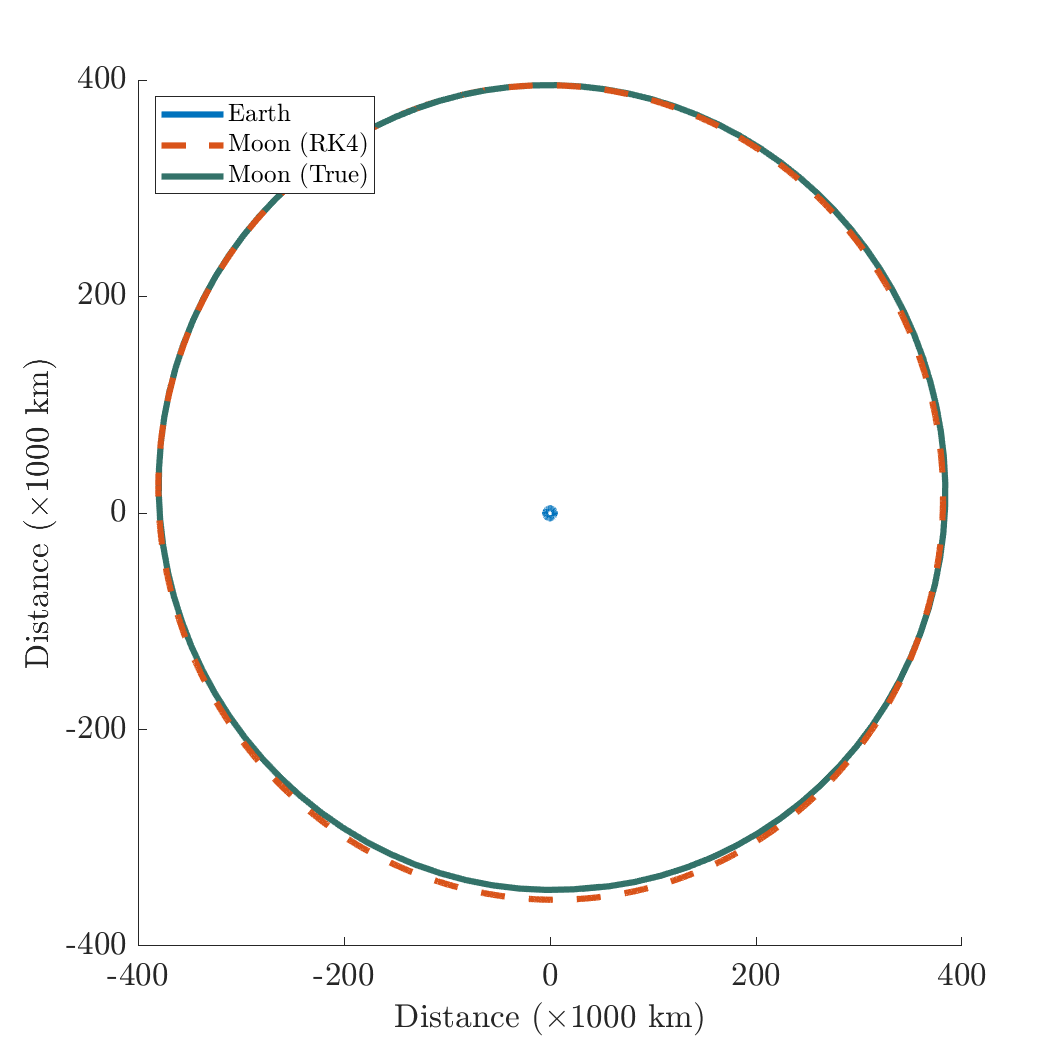
\includegraphics[height = 14cm]{Figures/Implementation/EM_Sys.png}
        \caption{Earth-Moon System with RK4 and \bm{$\Delta t$} = 238 \textbf{ s}}
        \label{em_sys}
    \end{figure}
    
    Figure \ref{em_sys} visualizes what the orbits of Earth and the Moon look like at a certain time. The circular paths represent the orbital movement corresponding to each body when the time step expands. For the moon, the gravitational force equation is used as an approximate to compare with the true orbit ,which results in a pretty accurate orbit as the approximate and the true measure of the Moon's orbit closely line up together. 
    
    \subsection{4-Body Simulation of The Solar System (N = 4)}
    \label{4_bod}
    Knowing how to implement the numerical methods into a two-body system (Earth and Moon System), it is possible to analyze further by increasing the number of bodies in a solar system. Instead of involving the Earth and the Moon, let's involve the Sun as the center of the solar system, Mercury, Earth, and Mars. The solar system will be expanded to a three-dimensional system. In addition to RK4, three more numerical methods (Forward Euler, Huen's, and KDK) will be implemented to show if there are different effects towards the four bodies. With the required equations and initial conditions utilized, the four-body system is plotted through each method, shown in Fig.\ref{fig:em system}:
    \begin{figure}[H]
        \centering
        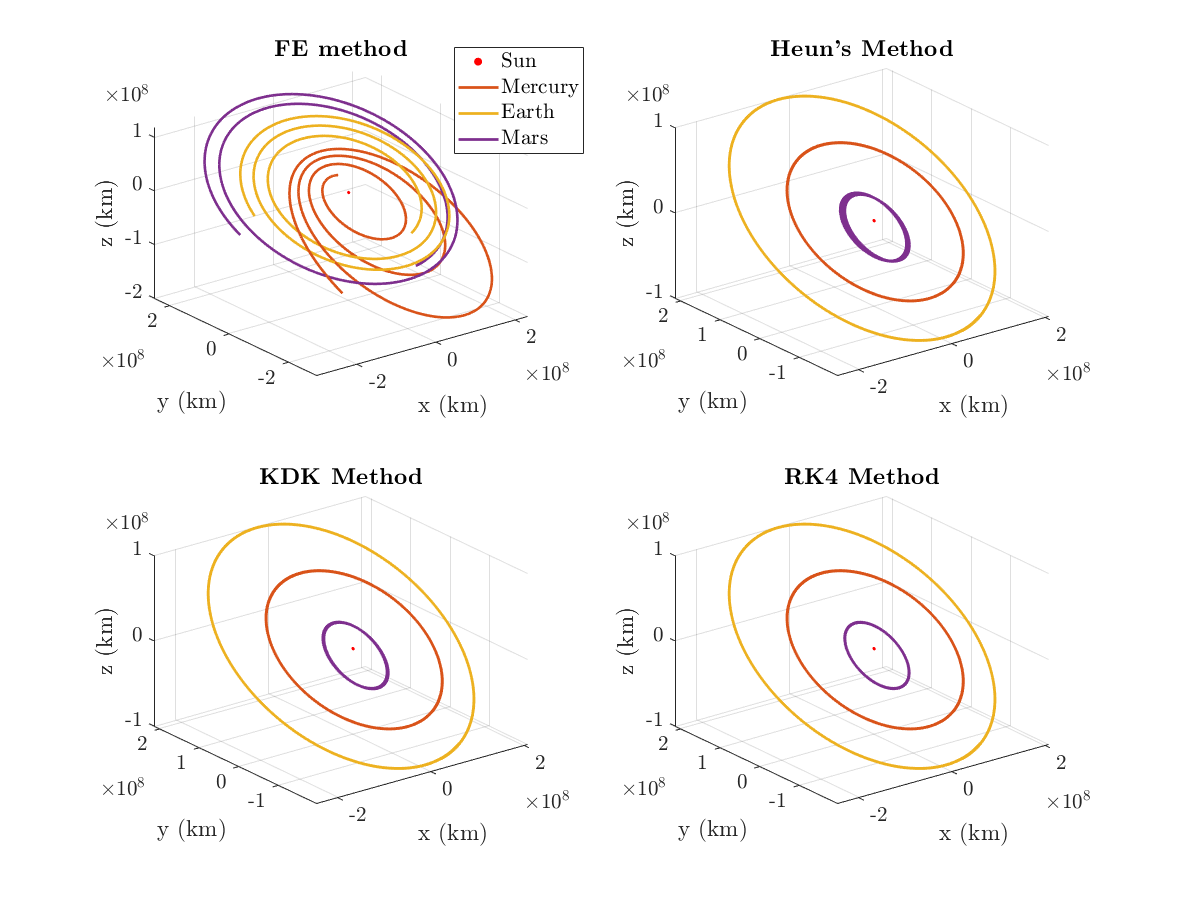
\includegraphics[height=13cm]{Figures/Implementation/4body system step100.png}
        \caption{4-Body System (N=4) for \bm{$\Delta t = 86400$} s}
        \label{fig:em system}
    \end{figure}
    The orbit of the solar system is plotted using the mass from NASA \cite{NASAplanet}, velocities and positions from the MATLAB command "\lstinline|planetEphemeris|" for the initial values. The time is set to be T = 1400 days, 12096 $\cdot$ $10^4$ seconds, so that each planet has at least two orbital periods. The time step is set to be 1400 steps, making the $\Delta t$ to be one day, 86400 seconds. From Fig. \ref{fig:em system}, it is observed that the FE method is not converging at all. The other three methods should be studied more in-depth to determine the best method for the solar system.
    
    \subsection{Method Accuracy}
    Since these four numerical methods are chosen to depict the solar system with the amount of N bodies, it goes furthermore to the extent where only one method is considered to be the best pick for accuracy. To do so, this paper will utilize the percent difference between the radius from the approximation methods and the true radius throughout the change of time. Then, the percent norm value of the difference for each method will be calculated to obtain a single number of error to compare the accuracy of each methods. This method is based on the convergence test method.
    \begin{equation}
        Error_{Mercury, method } =  \frac{||r_{\Delta t}-r_{true}||}{||r_{true}||}\cdot 100
        \label{eq:norm}
    \end{equation}
    The FE method is excluded from the error calculation since Fig. \ref{fig:em system} clearly showed a divergence for the FE method. Mercury is chosen as the representative of the error calculation since it has the most orbital periods among the other bodies at the given time. As mentioned earlier, the "\lstinline|PlanetEphemeris|" command is used to find the true radius for Mercury at each $\Delta t$. The same input described above is used to calculate the error. 
    Finally, the percent difference vs. time plot is made to visualize the trends of each method's accuracy and convergence, as shown in Fig. \ref{fig:accuracy}. 
    
\begin{figure}[H]
    \centering
    \includegraphics[width=0.9\textwidth]{Figures/Implementation/Mercury.png}
    \caption{Error Plot of Mercury for \bm{$\Delta t = 86400$} s}
    \label{fig:accuracy}
\end{figure}
    From Figure \ref{fig:accuracy},the three methods have shown to accurately measure the percent difference despite the Forward Euler method's failed attempt. It appears that the percent difference of Heun's method shows a larger wave, which is not close to the actual orbit. In contrast, the percent difference of KDK and RK4 method have drastically lower waves from the Heun's method, closer to the actual orbit. It is yet to determine which method is the best method through visual observation since the percent difference of KDK and RK4 method are very closed to each other. For further comparison, the percent norm value of the difference for each method, $Error_{Mercury, method }$, is calculated using equation \eqref{eq:norm}, as shown in Table \ref{tab:accuracy}.
    \begin{table}[H]
        \centering
        \caption{Error Calculation for Mercury}
        \begin{tabular}{c|c}
            \textbf{Approximation Method} & \textbf{Value (\%)} \\\hline\hline
             Heun's Method & 15.69\\
            Kick-Drift-Kick & 1.80\\
            RK4 & 0.57\\
            True Position& 0.00\\
        \end{tabular}
        \label{tab:accuracy}
    \end{table}
    In Table \ref{tab:accuracy}, the lower percent error indicates a higher accuracy. As it is observed from Fig. \ref{fig:accuracy}, the Huen's method shows the highest error. Finally, the table justifies that the RK4 method is the best method for accuracy, having the lowest error, RK4's percent error is 0.57 $\%$. 

    Now that the RK4 method is determined to be the optimal method for Solar system (or N-body system), the next step is to determine how $\Delta t$ can affect the accuracy and convergence of the N-body system with RK4 method.
    
\subsection{Time-Step Size Impact for a 2 Body System}
    While the numerical methods depict an N-body system, it is necessary to understand how the various time-step sizes can affect the numerical methods since stability is required to make a constant, orbital system without any changes. Let's say that there are two bodies with the same masses who encountered gravitational forces towards each other at a distance of km. Applying one of the methods (RK4 method) into the gravitational force of the two bodies, it is possible to create a plot for each time step $\Delta t$. Combining the method with each time step yields a plot shown in Figure \ref{step}:
     \begin{figure}[H]
        \centering
        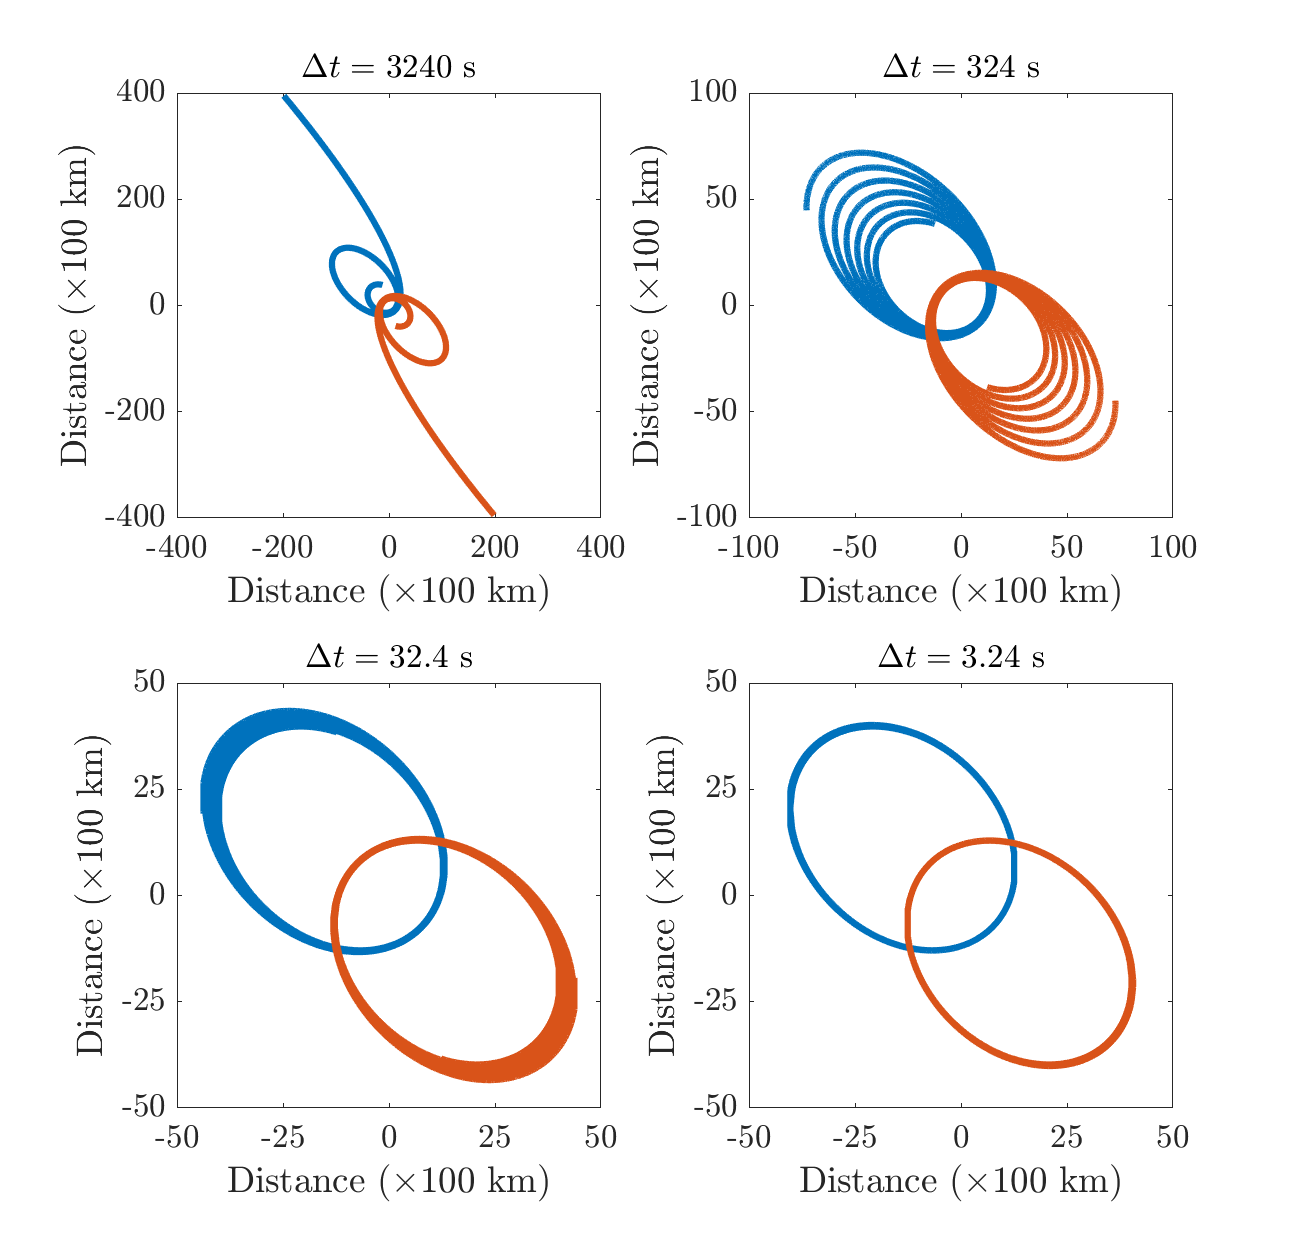
\includegraphics[height=14cm]{Figures/Implementation/N=2_Simulation.png}
        \caption{Step-Size Impact (RK4)}
        \label{step}
    \end{figure}
    
     From Figure \ref{step}, the orbits of the two bodies gradually become stable as $\Delta t$ decreases. For $\Delta t$= 3420s, the two bodies constantly orbit around each other until the extent where they lose balance, orbiting away from each other. Decreasing $\Delta t$ leads the orbits of the two bodies to slowly form a circular path until those paths become solidified and constant. Observing the results of the behavior of these bodies, it is indicated that having a smaller $\Delta t$ brings a bigger impact on the the orbital system. It is noted that Forward Euler method will require a smaller amount of $\Delta t$ because it is a first-order accurate. This method will also become time-consuming as well when plotting a large-scale system.
    
\section{Arenstorf Orbits}

In the 1960s, as the United States began to rapidly develop their human space program to put a man on the moon, a key issue presented itself in the form of the $N$-body problem: what trajectory would a human spacecraft need to take in order to intercept the Moon in orbit, but also return it back to Earth? Because this was a three body problem (Earth, Moon, and spacecraft), no analytical solution existed, so the trajectory needed to be evaluated numerically. In 1963, Richard Arenstorf, a NASA mathematician, derived the formulation of the Arenstorf orbits using a restriced three-bdoy problem. These orbits would form the basis of the Apollo Program's TLIs and Apollo 13's rescue-orbit trajectory.
    \subsection{Assumptions}
    Their are two key assumptions for deriving the Arenstorf orbits:
    \begin{enumerate}
        \item For a three body system made up of masses $m_1$, $m_2$, and $m_3$, have $m_2$ and $m_1$ exhibit planar circular orbits about the barycenter.
        \item For some $m_3$ with mass negligible in comparison to the $m_1$ and $m_2$, the gravitational impact of $m_3$ on $m_1$ and $m_2$ can be neglected.
    \end{enumerate}
    The Earth-Moon orbit exhibits a mean eccentricity of 0.054; thus the Earth-Moon System, the first assumption can be made. In addition, the Apollo Command Module and Lunar Lander weighed approximately 44 tons, which is 20 and 18 orders of magnitude less than the Earth and Moon, respectively. This means that the second assumption can also be made.
    \subsection{Derivation}
    Before the Arenstorf orbit equations can be derived, the following simplifications and relations need to be defined:
    \begin{tabularx}{\linewidth}{>{\leqnomode}XXX}
        \begin{equation}
        \begin{aligned}
            M = m_1 + m_2
            \label{Mass}
        \end{aligned}
        \end{equation}
        &        
        \begin{equation}
        \begin{aligned}
            \mu = \frac{m_2}{M}
            \label{mu}
        \end{aligned}
        \end{equation}
        &
        \begin{equation}
        \begin{aligned}
            \alpha = 1- \mu
            \label{alpha}
        \end{aligned}
        \end{equation}
    \end{tabularx}
    
    The subscripts 1, 2, and 3 will correspond to the Earth, Moon, and spacecraft properties, respectively. In addition, the terms "spacecraft" and "probe" will be used interchangeably. Now, using Equation (\ref{rddot}), the acceleration of the spacecraft can be written as
    \begin{equation}
	    \bm{\ddot{r}}_3 =  G \sum_{\substack{j=1}} ^{2} \frac{m_j (\bm{r}_j-\bm{r}_3)}{||\bm{r}_j-\bm{r}_3||^3}	
	    \label{gravity}
    \end{equation}
    where each vector $\bm{r}_j$ is drawn from the barycenter of the system to the $j^{th}$ body. Because the mass of the spacecraft $m_3$ is practically non-existent in comparison to the Earth and Moon masses, it does not need to be considered when finding the barycenter of this system. Additionally, because both the Earth and Moon are assumed to exhibit circular orbit paths and momentum must be conserved, both bodies will maintain the same angular velocity $\omega$ about the barycenter. Because gravity is the only force acting on these bodies, the acceleration due to gravity must be equal to the centripetal acceleration for both bodies. That is,
    \begin{align}
        \dot{r}_j &= r_j\frac{G m_{3-j}}{D^2} = r_j^2\omega^2,
        &
        \text{for } D &= |\bm{r}_1 + \bm{r}_2|
        \label{relation}
    \end{align}
    Kepler's third law, $\omega^2 = GM/D^3$,  is automatically obtained from this relation, since $m_{3-j} = MR_j/D$ via the conservation of momentum. This relation also proves that
    \begin{align}
        r_1 &= \mu D
        &
        r_2 = \alpha D
    \end{align}
    The positions of these bodies as a function of time $t$ can now be written as

    \begin{align}
        \bm{r}_1 &= \begin{bmatrix}
		\mu D \text{ cos } \omega t \\ \mu D \text{ sin } \omega t \\ 0
		\end{bmatrix}
		&
        \bm{r}_2 &= \begin{bmatrix}
		-\alpha D \text{ cos } \omega t \\ -\alpha D \text{ sin } \omega t \\ 0
		\end{bmatrix}
		&
		\bm{r}_3 &= \begin{bmatrix}
		x_3 \\
		y_3\\
		z_3\\
		\end{bmatrix}=
		\begin{bmatrix}
		D\cdot x\\
		D\cdot y\\
		D\cdot z\\
		\end{bmatrix}
		\label{radius}
    \end{align}
    Now, inserting Equations (\ref{mu}), (\ref{alpha}), (\ref{relation}), and (\ref{radius}) into Equation (\ref{gravity}) will yield::
    \begin{equation}
        \ddot{x}_3 = \frac{\alpha}{r^3_1}(\mu \text{ cos } \omega t-x) - \frac{\mu}{r^3_2}(\alpha \text{ cos } \omega t+x)
        \label{xdd_eq}
    \end{equation}
    \begin{equation}
        \ddot{y}_3 = \frac{\alpha}{r^3_1}(\mu \text{ sin } \omega t-y) - \frac{\mu}{r^3_2}(\alpha \text{ cos } \omega t+y)
        \label{ydd_eq}
    \end{equation}
    \begin{equation}
        \ddot{z}_3 = -\Bigg(\frac{\alpha}{r^3_1}+ \frac{\mu}{r^3_2}\Bigg)z_3
        \label{zdd_eq}
    \end{equation}
    Because the spacecraft's motion is $x$-$y$ planar, $z_3=0$ at all $t$, and thus Equation (\ref{zdd_eq}) can be neglected. The Equations are currently derived in the inertial reference frame, but can be made even simpler in the rotating (synodic) frame, where the Earth and Moon sit at fixed positions in the frame and all motion is represented by the spacecraft \cite{R3BP}. To do this, $x^*$, $y^*$, and $z^*$, can be introduced as synodic coordinates, where\\
    \begin{tabularx}{\linewidth}{>{\leqnomode}XX}
        \begin{equation}
        \begin{aligned}
            x = x^* \text{ cos } \omega t - y^* \text{ sin } \omega t 
            \label{x_star}
        \end{aligned}
        \end{equation}
        &        
        \begin{equation}
        \begin{aligned}
            y = x^* \text{ sin } \omega t + y^* \text{ cos } \omega t 
            \label{y_star}
        \end{aligned}
        \end{equation}
    \end{tabularx}
    Finally, Equations (\ref{x_star}) and (\ref{y_star}) can be inserted into Equations (\ref{xdd_eq}) and (\ref{ydd_eq}) to get the Arenstorf Orbit Equations such that
    \begin{equation}
        \ddot{x}^*_3 = 2\dot{y}^* + x^* +\frac{\alpha}{r^3_1}(\mu-x^*) - \frac{\mu}{r^3_2}(\alpha+x^*)
        \label{xdd_Aren}
    \end{equation}
    \begin{equation}
        \ddot{y}^*_3 = -2\dot{x}^* + \Bigg(1 -\frac{\alpha}{r^3_1} - \frac{\mu}{r^3_2}\Bigg)y^*
        \label{ydd_Aren}
    \end{equation}
    where
    \begin{equation}
        r_1 = D\sqrt{(x^*-\mu)^2+(y^*)^2)}
        \label{r_1_D}
    \end{equation}
    \begin{equation}
        r_2 = D\sqrt{(x^*+\alpha)^2+(y^*)^2)}
        \label{r_2_D}
    \end{equation}
    Equations (\ref{xdd_Aren}) and (\ref{ydd_Aren}) will form the basis of the $N$-body problem solved in the \ref{Stable_O}.
    \subsection{Stable Orbits}
    \label{Stable_O}
    Using the Arenstorf orbit equations, stable and periodic orbital paths for the probe in the Earth-Moon system can be found. The numerical method used to represent this system will, as demonstrated earlier, have a profound effect on the accuracy of the represented Arenstorf orbit. The following initial conditions, which correspond to the most widely available and well known Arenstorf solution, can be used to verify the approximation accuracy:
    \begin{align}
	    \bm{r}_1 &= \begin{bmatrix}
		-\mu D \\ 0 \\ 0
	    \end{bmatrix}
        &
	    \bm{r}_2 &= \begin{bmatrix}
		 \alpha D\\ 0 \\ 0
	    \end{bmatrix}
	    &
	    \bm{r}_3 &= \begin{bmatrix}
		 0.994 \cdot \alpha D\\ 0 \\ 0
	    \end{bmatrix}
	    \label{r_Ar}
    \end{align}
    \begin{align}
	    \dot{\bm{r}}_1 &= \begin{bmatrix}
		0 \\ 0 \\ 0
	    \end{bmatrix}
        &
	    \dot{\bm{r}}_2 &= \begin{bmatrix}
		0\\ 0 \\ 0
	    \end{bmatrix}
	    &
	    \dot{\bm{r}}_3 &= \begin{bmatrix}
		0\\ -2001.585 \\ 0
	    \end{bmatrix}
	    \label{vel_Ar}
    \end{align}
    The $\dot{r}$ components correspond to the velocity of the three bodies in the synodic frame. In the inertial frame, $(\dot{r}_y)_1=-\omega \mu D$ and $(\dot{r}_y)_2 = \omega \alpha D$. With these initial conditions and the Arenstorf orbit equations, Forward Euler, Heun's Method, KDK, and RK4 can be used to approximate the probe path, plotted in Figure \ref{Aren}.
    \begin{figure}[H]
        \centering
        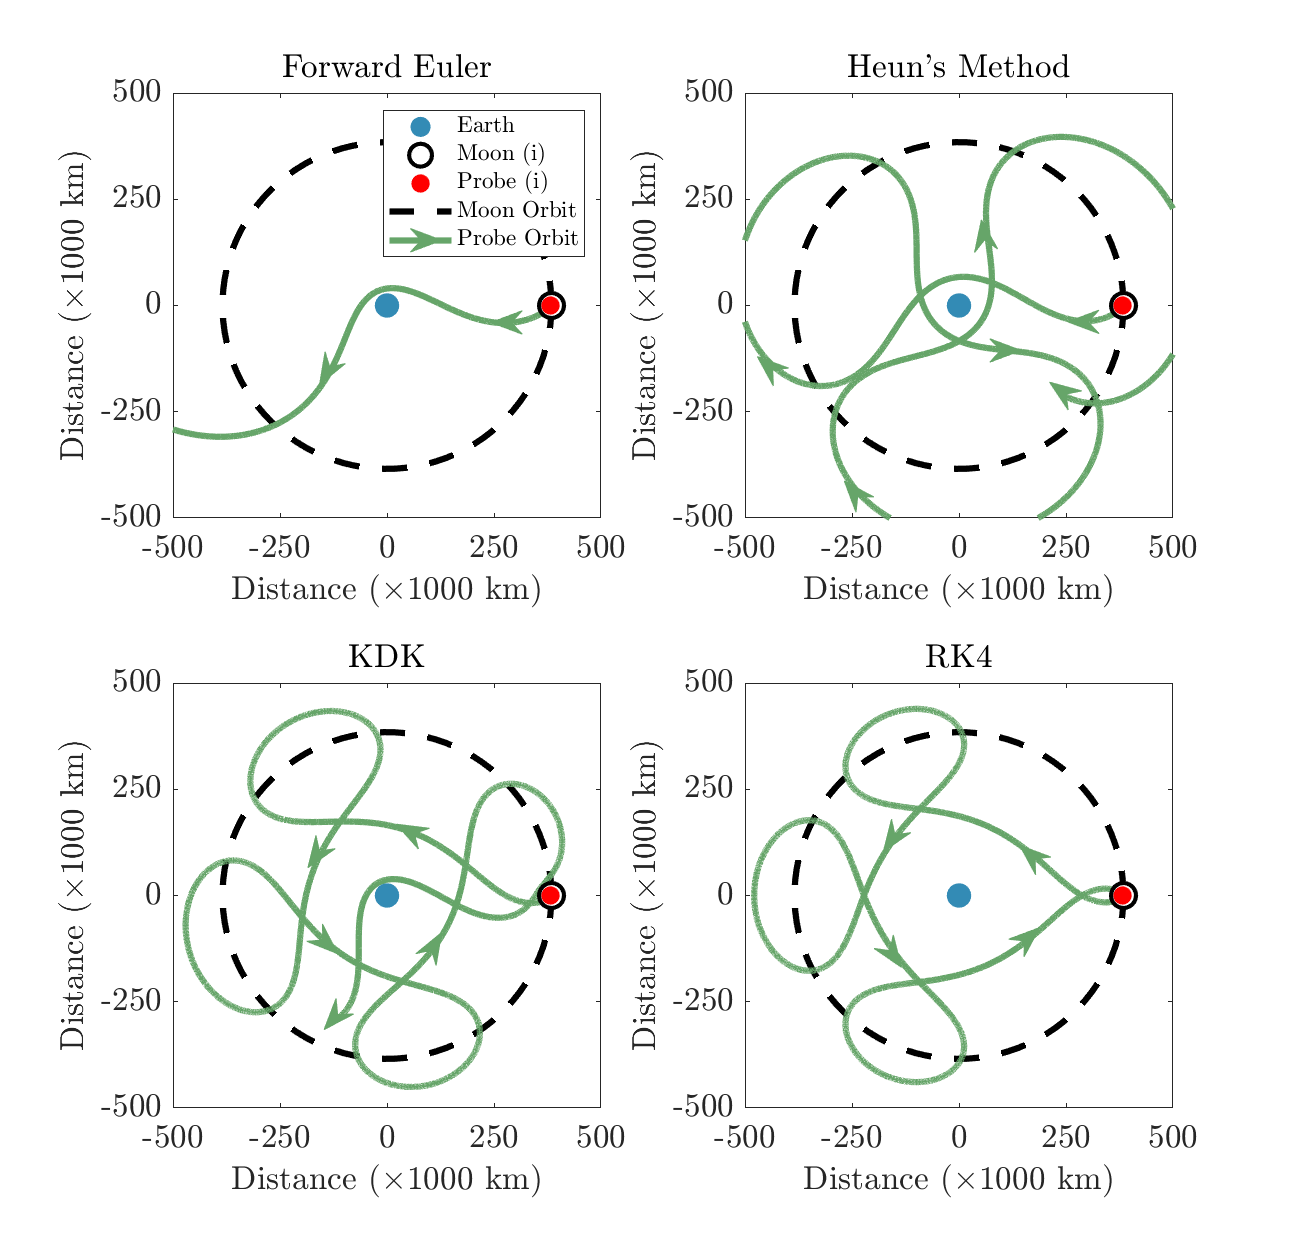
\includegraphics[height = 14cm]{Figures/Arenstorf/Arenstorf.png}
        \caption{Estimations of Arenstorf Orbits for Various Numerical Methods and \bm{$\Delta t = 158$} \textbf{ s}}
        \label{Aren}
    \end{figure}
    As can be seen, only RK4 demonstrates a stable, periodic orbital path, and identically matches the Arenstorf solution. The Forward Euler Method yields both an unstable and non-periodic solution; the probe is jettisoned from the Earth-Moon system, and does not represent the Arenstorf solution. Heun's Method and KDK both exhibit stable orbital paths, with the probe remaining under the gravitational influence of the Earth-Moon system, but both methods do not exhibit periodic orbits.
    \subsubsection{RK4 Stability Validation}
    Because RK4 was the only numerical method that accurately depicted the well-known Arenstorf orbit, it was further investigated to determine its error over $n$ orbital periods. The orbit is only periodic of the initial conditions shown in Equations \eqref{r_Ar} and \eqref{vel_Ar} are replicated at the end of each period. After one periodic orbit, the probe arrives at roughly the same initial position with the same initial velocity, albeit with minimal error. However, as the number of orbital periods $n$ increases, the error associated with the ending conditions of each orbit increases, which should eventually create a non-periodic unstable orbit. This error and instabililty can be seen in Figure (\ref{RK4_Period})
        \begin{figure}[H]
            \centering
            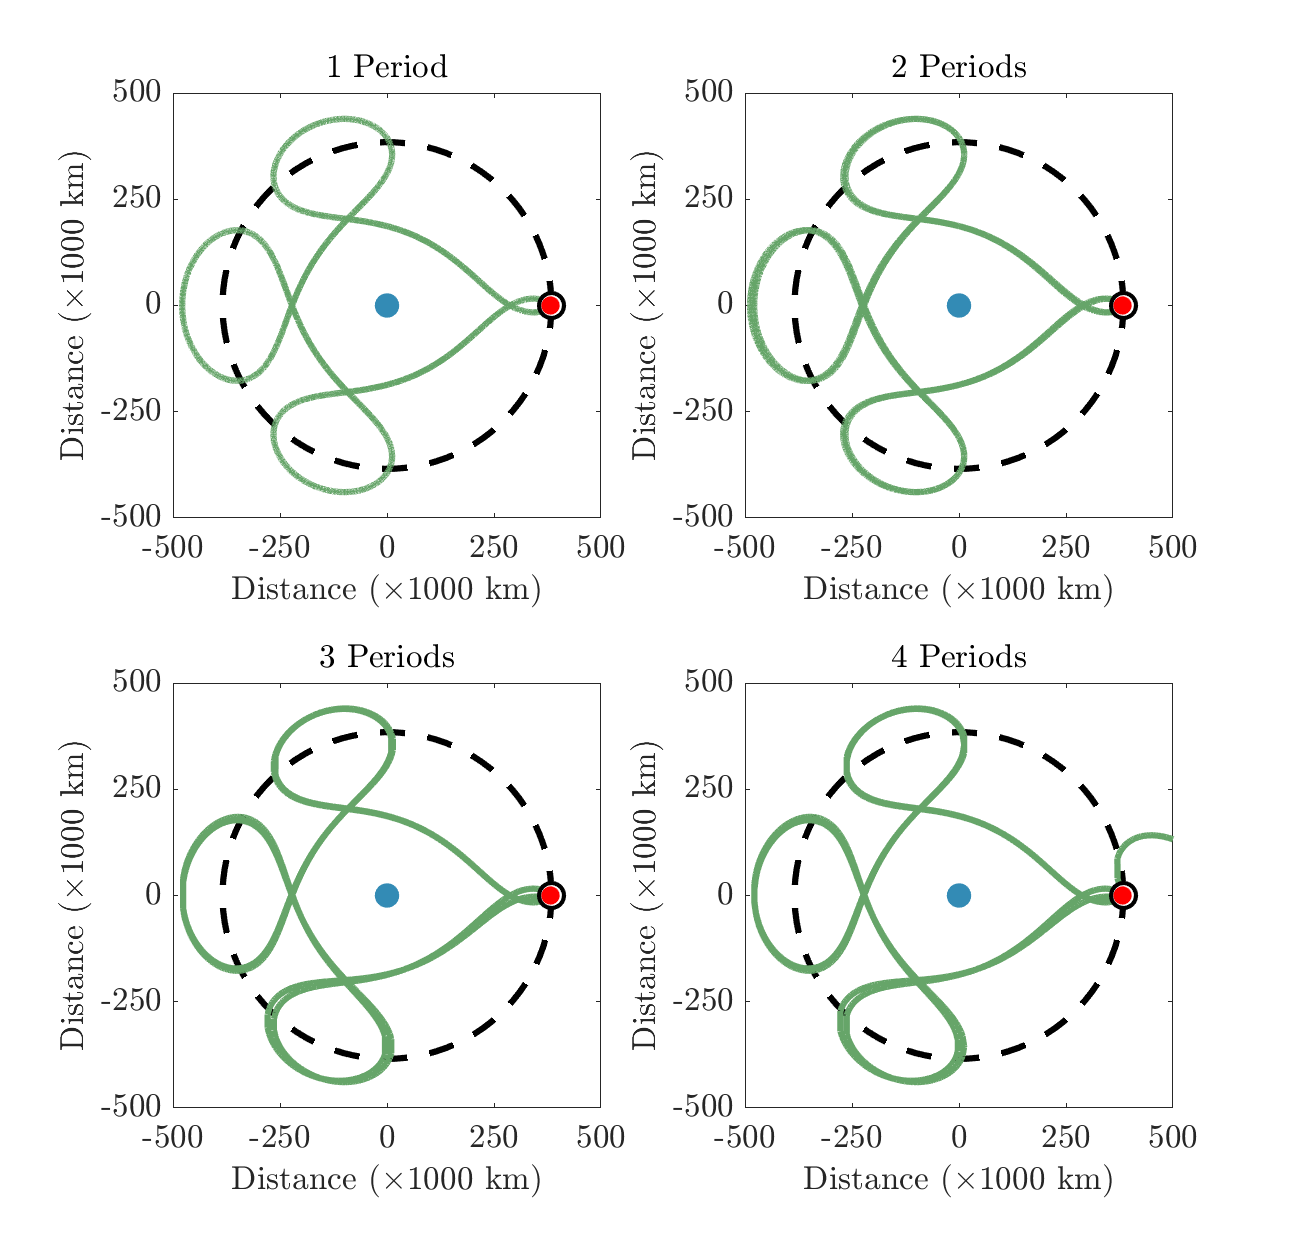
\includegraphics[height = 14cm]{Figures/Arenstorf/Aren_Stability.png}
            \caption{Error and Instability of RK4 Arenstorf Orbits for \bm{$n$} Orbital Periods and \bm{$\Delta t = 158$} \textbf{ s}}
            \label{RK4_Period}
        \end{figure}
    As mentioned earlier, the RK4 estimation of a single Arenstorf orbit is practically perfect, and the error/ instability cannot even be inferred from the plot. Over $n=2$ orbital periods, the probe's orbital path starts to look a little bit different, and starts to trace out a slightly different path for every $nth$ orbit. For $n=3$, it becomes clear that the approximated orbit is starting to become non-periodic and displaying some signs of instability; there are small (but clear) gaps that have formed inbetween the traced orbits. For $n=4$, the approximated Arenstorf orbit is both non-periodic and unstable, as the probe is shown completely leaving the Earth-Moon system. At this stage, the final velocity of the third orbit is too high an estimate for the Moon to curve the probe back towards the barycenter. To counteract this, $\Delta t$ would need to shrink in size and the stable initial conditions would need to be calculated with more significant figures.
    \subsection{Translunar Insertion}
    
    While it is a stable and periodic orbit, the common Arenstorf Orbit solution represented in Figure \ref{RK4_Period} is not feasible to use for a TLI. The entire purpose of Arenstorf's original research and derivation was to find a periodic orbit that could be used to intercept the Moon from Earth, but also offer a return path; at it's closest point, the common solution probe path is still 170,000 km away from Earth. As a result, another path with different initial conditions needed to be found. Arenstorf's original research paper details a "5-lobed" stable orbit (which was used for the Apollo TLIs), but does not mention the initial conditions needed to establish it \cite{Aren_paper}. With the framework developed in Section \ref{Stable_O}, the Apollo TLI can be found iteratively by varying the initial conditions until a stable, periodic orbit that replicates the "5 lobes" is established. The Apollo TLI was eventually found, with initial conditions
    \begin{align}
	    \bm{r}_3 &= \begin{bmatrix}
		1.011\alpha D \\ 0 \\ 0
	    \end{bmatrix}
        &
	    \bm{\dot{r}}_3 &= \begin{bmatrix}
		0 \\ -1346.566 \\ 0
	    \end{bmatrix}
    \end{align} 
    This iterative solution was verified by plotting the Arenstorf orbit, which can be seen in Figure \ref{TLI}.
    \begin{figure}[H]
        \centering
        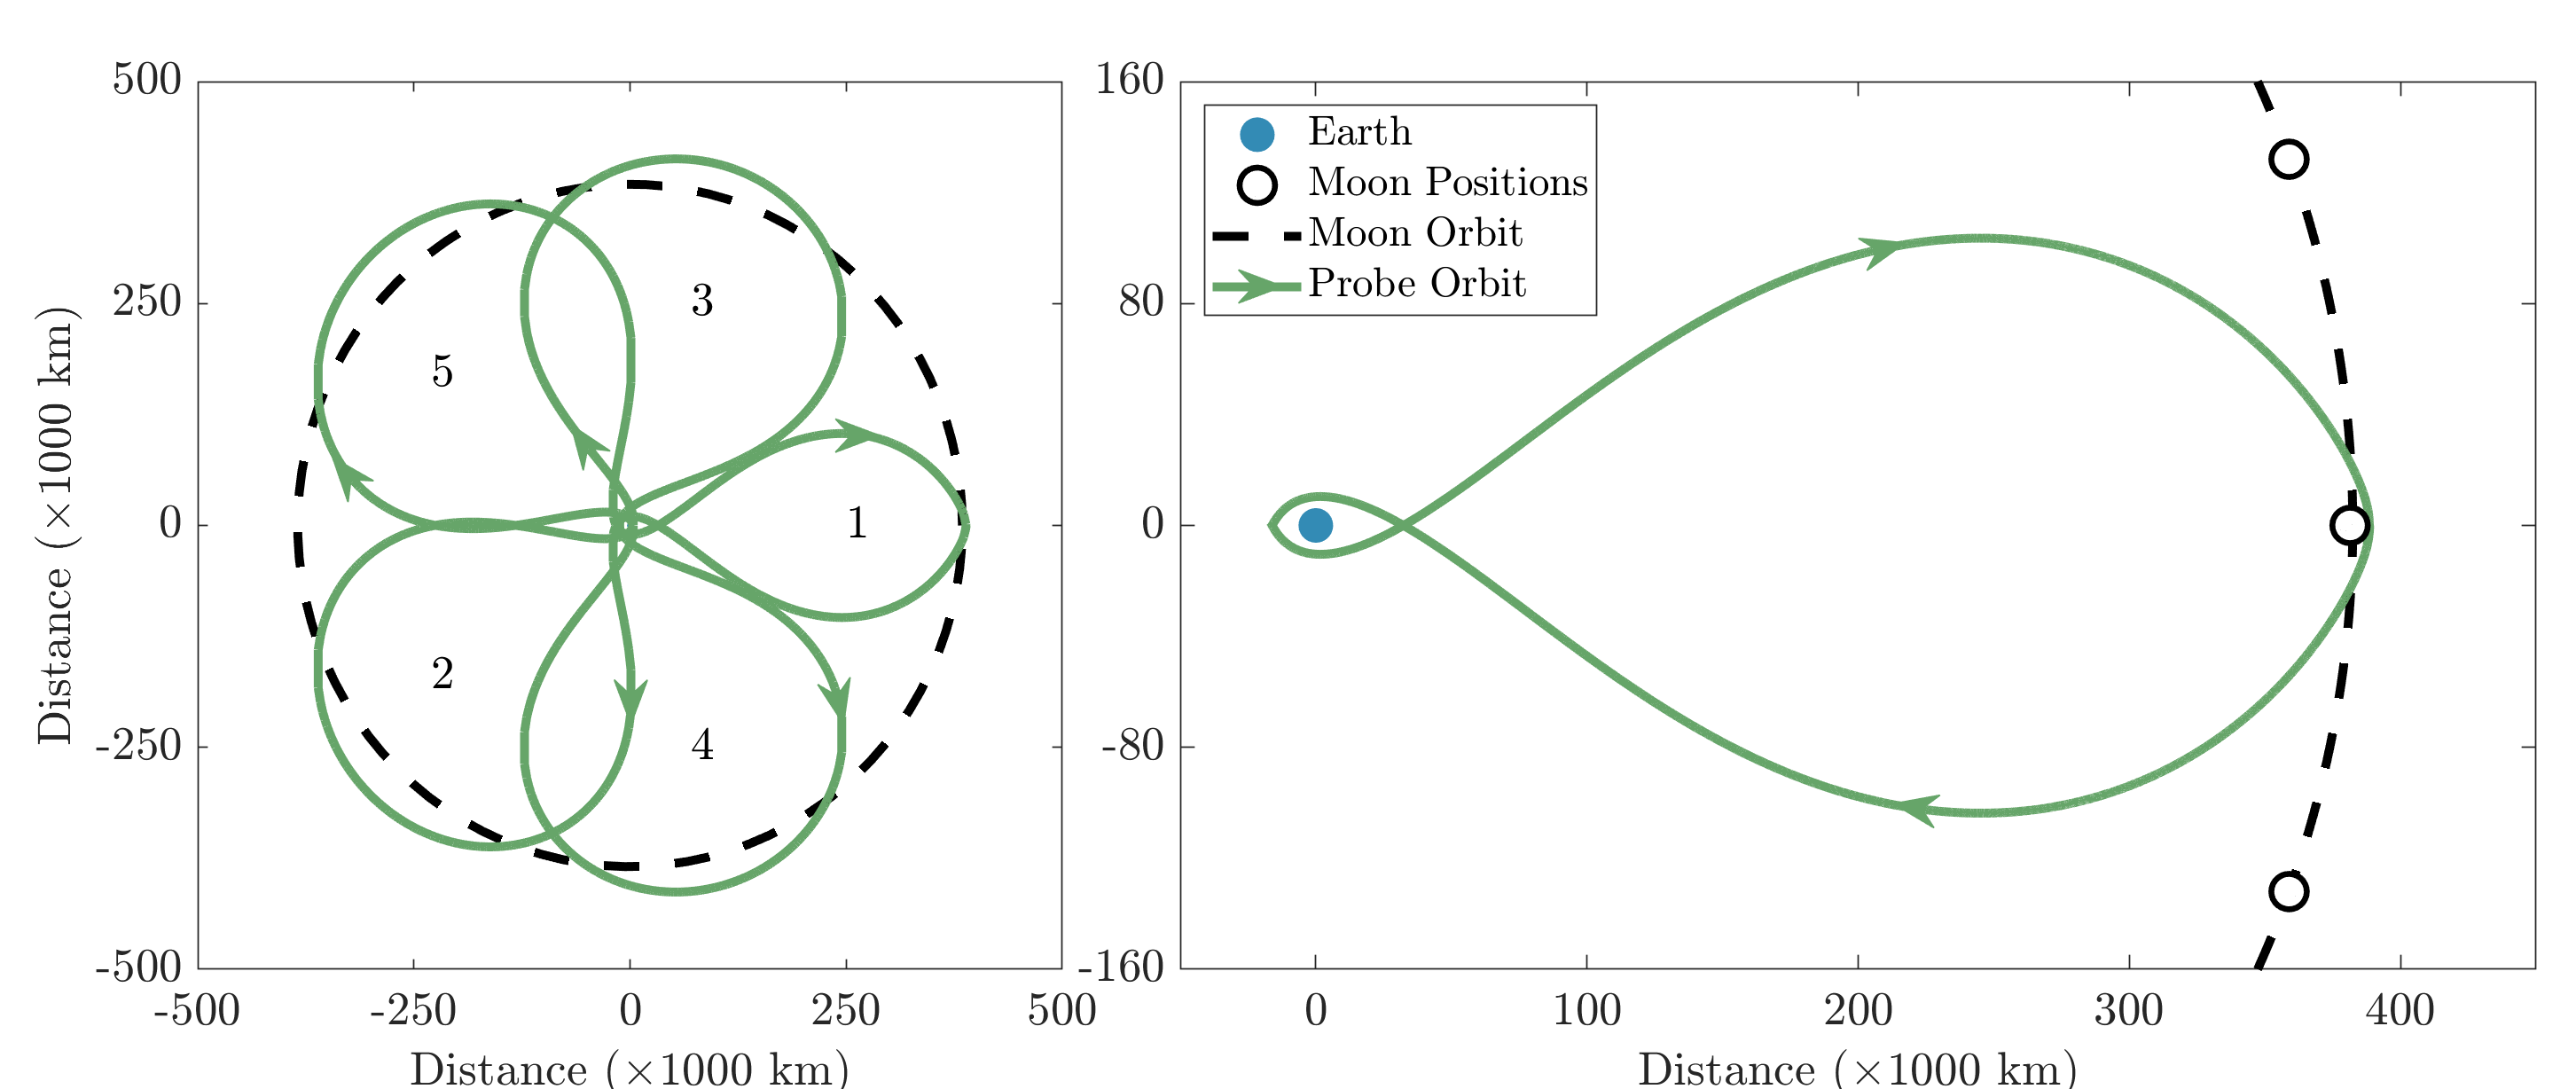
\includegraphics[height = 7cm]{Figures/Arenstorf/TLI.png}
        \caption{Apollo 13 TLI solved using Arenstorf Orbit Equations and RK4}
        \label{TLI}
    \end{figure}
    The left plot shows the stable orbit over an entire period, while the right plot shows the path that a probe/ spacecraft would take when leaving Earth, intercepting the Moon, and then returning to Earth. The minimum distance between the probe's orbit path and the Earth's surface is less than 1900 km, which puts it in Low Earth Orbit (LEO). Additionally, at this point, the probe's velocity is roughly 10.25 km/s, which is ~1.5\% less than the actual orbital velocity achieved during the Apollo 11 mission in LEO \cite{Apollo}. This demonstrates that the RK4 implementation was accurate enough to find the stable Arenstorf TLI with phenomenal accuracy when compared to the real flight data.
\section{Conclusions}
After implementing various $N$-body systems, it is clear that RK4 works substantially better than the other methods investigated. For larger $\Delta t$ values over longer periods of time, RK4 managed to generate substantially more accurate orbital paths in comparison to the Forward Euler, Heun's, and even KDK methods, as can be seen in Figure \ref{fig:accuracy}. For the stable implemented example shown in Figure \ref{step}, RK4 can use a $\Delta t$ roughly three times larger that KDK and Heun's Method while still giving a more accurate result. The error analysis shown in Figure \ref{fig:accuracy} further validates RK4's superior performance. While decreasing $\Delta t$ can improve the predicted orbit accuracy, using a higher order-of-accuracy method is far more effective and time-efficient at reducing error, even though that method might be more difficult to implement.

Further improvements and analysis can simulate planetary motion for greater $N$, such as for the Solar System. Additionally, more complex Arenstorf systems, such as the Sun-Earth System, could be used to investigate the path that SpaceX's Starman took to enter heliocentric from Earth or Voyager's initial path to leave the Solar System. 
\pagebreak

\bibliography{sample}
\pagebreak
\begin{quote}
    \begin{lstlisting}
    %% Initialize Values
clc
clear all
%Earth %Moon %Other Satellites/ Capsules

N = 2; %number of bodies (<= 5)

Time = 900; %Total time elapsed (hours)
step = 1000*[1 10 100 1000]; %Total number of points

%Change up to the Nth Initial Body Position
x1_i = [-1.23e7 3.84e7]; %Initial 1st Body Position (m)
x2_i = [1.23e7 -3.84e7]; %Initial 2nd Bodu Position (m)

%Change up to the Nth Initial Body Velocity
v1_i = [-380 120]; %Initial 1st Body Velocity (m/s)
v2_i = [380 -120]; %Initial 2nd Body Velocity (m/s)

%Change up to the Nth Initial Body Mass
m_1 = 5.972e23; %1st Body Mass (kg)
m_2 = 5.972e23; %2nd Body Mass (kg)

%%


for alpha = 1:length(step)
    steps = step(alpha);
    x = zeros(steps, 4);
    v = zeros(steps, 4);
    
    t = 0;
    dt = Time*3600/steps; %time step (s)
    mass = [m_1, m_2];
    x(1,:) = [x1_i, x2_i];
    v(1,:) = [v1_i, v2_i];
    for k = 1:steps
        t = t + dt;
        for i = 1:N
            x_i = x(k, ((i-1)*2+1):i*2); %Get the position in m
            v_i = v(k, ((i-1)*2+1):i*2); %Get the vel in m/s

            x_ip1 = x_i;
            v_ip1 = v_i;
            const = 0;
            for j = 1:N
                if j ~= i
                    x_j = x(k,((j-1)*2+1):j*2);
                    
                    k1x = dX_dT(mass(1,j), x_i, x_j, v_i);
                    k1v = dV_dT(mass(1,j), x_i, x_j);
                    
                    k2x = dX_dT(mass(1,j), x_i+dt*k1x/2, x_j, v_i+dt*k1v/2);
                    k2v = dV_dT(mass(1,j), x_i + dt*k1x/2, x_j);
                    
                    k3x = dX_dT(mass(1,j), x_i+dt*k2x/2, x_j, v_i+dt*k2v/2);
                    k3v = dV_dT(mass(1,j), x_i + dt*k2x/2, x_j);
                    
                    k4x = dX_dT(mass(1,j), x_i+dt*k3x, x_j, v_i+dt*k3v);
                    k4v = dV_dT(mass(1,j), x_i + dt*k3x, x_j);

                    x_ip1 = x_ip1 + dt/6*(k1x+2*k2x+2*k3x+k4x);
                    v_ip1 = v_ip1 + dt/6*(k1v+2*k2v+2*k3v+k4v);
                end
            end
            x(k+1, ((i-1)*2+1):i*2) = x_ip1;
            v(k+1, ((i-1)*2+1):i*2) = v_ip1;
        end
    end
    figure(1568)
    subplot(2,2,alpha)
    plot(x(:,1)/10e5,x(:,2)/10e5,'LineWidth',3)
    hold on
    plot(x(:,3)/10e5,x(:,4)/10e5,'LineWidth',3)
    hold on
    xlabel('Distance ($\times100$ km)','interpreter','latex','fontsize',16)
    ylabel('Distance ($\times100$ km)','interpreter','latex','fontsize',16)
    if alpha==1
        set(gcf, 'PaperUnits', 'centimeters')
        set(gcf, 'PaperSize', [22 22])
        set(gcf, 'Units', 'centimeters' )
        set(gcf, 'Position', [20 0 22 22])
        set(gcf, 'PaperPosition', [0 0 22 22])
        xlim([-400 400])
        ylim([-400 400])
        x_val = [-400 -200 0 200 400];
        y_val = [-400 -200 0 200 400];
        set(gca,'xtick', x_val, 'xticklabel', num2str(x_val.'))
        set(gca,'ytick', y_val, 'yticklabel', num2str(y_val.'))
        set(gca, 'TickLabelInterpreter','latex', 'fontsize', 16)
        title('$\Delta t = 3240$ s','interpreter','latex','fontsize',16)
    elseif alpha ==2
        x_val = [-100 -50 0 50 100];
        y_val = [-100 -50 0 50 100];
        set(gca,'xtick', x_val, 'xticklabel', num2str(x_val.'))
        set(gca,'ytick', y_val, 'yticklabel', num2str(y_val.'))
        set(gca, 'TickLabelInterpreter','latex', 'fontsize', 16)
        title('$\Delta t = 324$ s','interpreter','latex','fontsize',16)
    elseif alpha ==3
        x_val = [-50 -25 0 25 50];
        y_val = [-50 -25 0 25 50];
        set(gca,'xtick', x_val, 'xticklabel', num2str(x_val.'))
        set(gca,'ytick', y_val, 'yticklabel', num2str(y_val.'))
        set(gca, 'TickLabelInterpreter','latex', 'fontsize', 16)
        title('$\Delta t = 32.4$ s','interpreter','latex','fontsize',16)
    elseif alpha ==4
        x_val = [-50 -25 0 25 50];
        y_val = [-50 -25 0 25 50];
        set(gca,'xtick', x_val, 'xticklabel', num2str(x_val.'))
        set(gca,'ytick', y_val, 'yticklabel', num2str(y_val.'))
        set(gca, 'TickLabelInterpreter','latex', 'fontsize', 16)
        title('$\Delta t = 3.24$ s','interpreter','latex','fontsize',16)
    end
end
set(gcf, 'PaperPositionMode', 'auto')
saveas(gcf,'N=2_Simulation.png')
%%
function ans = dV_dT(m_j, r_i, r_j)
    G = 6.67430e-11; %Grav Const (m^3/(kg.s^2))
    ans = G*m_j*(r_j-r_i)/((norm(r_j-r_i))^3);
end
%%
function ans = dX_dT(m_j, r_i, r_j, v_i)
    if m_j == 0
        ans = 0;
    else
    ans = v_i;
    end
end
    \end{lstlisting}
\end{quote}


\begin{quote}
    \begin{lstlisting}
    %% Initialize Values

clc
clear all
close all
%Earth %Moon %Other Satellites/ Capsules

N = 2; %number of bodies (<= 5)

Time = 660; %Total time elapsed (hours)
steps = 100000; %Total number of points

%Change up to the Nth Initial Body Position

[xE_i, vE_i] = planetEphemeris(juliandate(1969,7,16),'EarthMoon','Earth');
[xM_i, vM_i] = planetEphemeris(juliandate(1969,7,16),'EarthMoon','Moon');

%Find Proper Rotation

z_rot_vec = [xM_i(1) xM_i(2) 0];
y_rot_vec = [xM_i(1) 0 xM_i(3)];
x_rot_vec = [0 xM_i(2) xM_i(3)];
ang_x = acosd(dot(xM_i, x_rot_vec)/norm(xM_i)/norm(x_rot_vec));
ang_y = acosd(dot(xM_i, y_rot_vec)/norm(xM_i)/norm(y_rot_vec));
ang_z = acosd(dot(xM_i, z_rot_vec)/norm(xM_i)/norm(z_rot_vec));

syms x y z real
Rz = [cosd(z) -sind(z) 0; sind(z) cosd(z) 0; 0 0 1];
Ry = [cosd(y) 0 sind(y); 0 1 0; -sind(y) 0 cosd(y)];
Rx = [1 0 0; 0 cosd(x) -sind(x); 0 sind(x) cosd(x)];
Rot = subs(Rx*Rz,[x,z],[ang_x, ang_z]);

xE_i = 1000*xE_i;
vE_i = 1000*vE_i;
xM_i = 1000*xM_i;
vM_i = 1000*vM_i;

x_b1 = xE_i + xE_i/norm(xE_i);%*sqrt(1000000); %Initial 1st Body Position (m)
x_b2 = [3e7 3e7]; %Initial 2nd Body Position (m)
x_b3 = [0 0]; %Initial 3rd Body Position (m)

%Change up to the Nth Initial Body Velocity

v_b1 = [0 0 0]; %Initial 1st Body Velocity (m/s)
v_b2 = [50 0]; %Initial 2nd Body Velocity (m/s)
v_b3 = [0 0]; %Initial 3rd Body Velocity (m/s)

%Change up to the Nth Initial Body Mass
m_E = 5.97237e24; %Earth Mass (kg)
m_M = 7.34767309e22; %Moon Mass (kg)

m_b1 = 20000; %Initial 1st Body Mass (kg)
m_b2 = 2.972e7; %Initial 2nd Body Mass (kg)
m_b3 = 0; %Initial 3rd Body Mass (kg)
    
%%
x = zeros(steps, N*3);
v = zeros(steps, N*3);

xpos_m = [0 0 0];
vpos_m = [0 0 0];

xpos_e = [0 0 0];
vpos_e = [0 0 0];


if N == 2
    mass = [m_E, m_M];
    x(1,:) = [xE_i, xM_i];
    v(1,:) = [vE_i, vM_i];
elseif N == 3
    mass = [m_E, m_M, m_b1];
    x(1,:) = [xE_i, xM_i, x_b1];
    v(1,:) = [vE_i, vM_i, v_b1];
elseif N ==4
    mass = [m_E, m_M, m_b1, m_b2];
    x(1,:) = [xE_i, xM_i, x_b1, x_b2];
    v(1,:) = [vE_i, vM_i, v_b1, v_b2];
else
    mass = [m_E, m_M, m_b1, m_b2, m_b3];
    x(1,:) = [xE_i, xM_i, x_b1, x_b2, x_b3];
    v(1,:) = [vE_i, vM_i, v_b1, v_b2, v_b3];
end


t = 0;
dt = Time*3600/steps; %time step (s)


for k = 1:steps
    t = t + dt;
    for i = 1:N
        x_i = x(k, ((i-1)*3+1):i*3); %Get the position in m
        v_i = v(k, ((i-1)*3+1):i*3); %Get the vel in m/s
        
        x_ip1 = x_i;
        v_ip1 = v_i;
        const = 0;
        for j = 1:N
            if j ~= i
                x_j = x(k,((j-1)*3+1):j*3);
                k1x = dx_dt(mass(1,j), x_i, x_j, v_i);
                k1v = dv_dt(mass(1,j), x_i, x_j);
                k2x = dx_dt(mass(1,j), x_i+dt*k1x/2, x_j, v_i+dt*k1v/2);
                k2v = dv_dt(mass(1,j), x_i + dt*k1x/2, x_j);
                k3x = dx_dt(mass(1,j), x_i+dt*k2x/2, x_j, v_i+dt*k2v/2);
                k3v = dv_dt(mass(1,j), x_i + dt*k2x/2, x_j);
                k4x = dx_dt(mass(1,j), x_i+dt*k3x, x_j, v_i+dt*k3v);
                k4v = dv_dt(mass(1,j), x_i + dt*k3x, x_j);
                
                x_ip1 = x_ip1 + dt/6*(k1x+2*k2x+2*k3x+k4x);
                v_ip1 = v_ip1 + dt/6*(k1v+2*k2v+2*k3v+k4v);
            end
        end
        x(k+1, ((i-1)*3+1):i*3) = x_ip1;
        v(k+1, ((i-1)*3+1):i*3) = v_ip1;
        if k > 1
            if N ==2
                if x_i(1) < 10e2
                    xpos_m = [x_i(1) x_i(2) x_i(3)];
                    vpos_m = [v(k-1,4) v(k-1,5) v(k-1,6)];
                    xpos_e = [x(k-1,1) x(k-1,2) x(k-1,3)];
                    vpos_e = [v(k-1,1) v(k-1,2) v(k-1,3)];
                end
            end
        end
    end
end

%% 3D View
figure(1)
for i=1:N
    if i == 1
        plot3(x(:,(i-1)*3+1),x(:,(i-1)*3+2),x(:,(i-1)*3+3),'LineWidth',3)
        hold on
    end
    if i ~=3
        if i ~=1
            plot3(x(:,(i-1)*3+1),x(:,(i-1)*3+2),x(:,(i-1)*3+3),'--','LineWidth',3)
            hold on
        end
    else
        plot3(x(:,(i-1)*3+1),x(:,(i-1)*3+2),x(:,(i-1)*3+3),'k','--','LineWidth',3)
        hold on
    end
    if i==1
        set(gcf, 'PaperUnits', 'centimeters')
        set(gcf, 'PaperSize', [18 18])
        set(gcf, 'Units', 'centimeters' )
        set(gcf, 'Position', [8 2 18 18])
        set(gcf, 'PaperPosition', [0 0 18 18])
    end
end
xlabel('Distance (Km)')
ylabel('Distance (Km)')
zlabel('Distance (Km)')
legend('Earth','Moon(approx)','Moon(true)')
%% True Data
xtrue = zeros(steps/100,3);
for i = 1:steps/100
    [xM_t, vM_t] = planetEphemeris(juliandate(1969,7,27.922*100/steps*(i-1)+1),'EarthMoon','Moon');
    xtrue(i,:) = xM_t*1000;
end
%%
plot3(xtrue(:,1),xtrue(:,2),xtrue(:,3),'-','LineWidth',3,'Color',[0.2, 0.4470, 0.410])
%% Planar

xE_i = xE_i*Rot;
vE_i = vE_i*Rot;
xM_i = xM_i*Rot;
vM_i = vM_i*Rot;


if N == 2
    mass = [m_E, m_M];
    x(1,:) = [xE_i, xM_i];
    v(1,:) = [vE_i, vM_i];
elseif N == 3
    mass = [m_E, m_M, m_b1];
    x(1,:) = [xE_i, xM_i, x_b1];
    v(1,:) = [vE_i, vM_i, v_b1];
elseif N ==4
    mass = [m_E, m_M, m_b1, m_b2];
    x(1,:) = [xE_i, xM_i, x_b1, x_b2];
    v(1,:) = [vE_i, vM_i, v_b1, v_b2];
else
    mass = [m_E, m_M, m_b1, m_b2, m_b3];
    x(1,:) = [xE_i, xM_i, x_b1, x_b2, x_b3];
    v(1,:) = [vE_i, vM_i, v_b1, v_b2, v_b3];
end

t = 0;
dt = Time*3600/steps; %time step (s)


for k = 1:steps
    t = t + dt;
    for i = 1:N
        x_i = x(k, ((i-1)*3+1):i*3); %Get the position in m
        v_i = v(k, ((i-1)*3+1):i*3); %Get the vel in m/s
        
        x_ip1 = x_i;
        v_ip1 = v_i;
        const = 0;
        for j = 1:N
            if j ~= i
                x_j = x(k,((j-1)*3+1):j*3);
                k1x = dx_dt(mass(1,j), x_i, x_j, v_i);
                k1v = dv_dt(mass(1,j), x_i, x_j);
                k2x = dx_dt(mass(1,j), x_i+dt*k1x/2, x_j, v_i+dt*k1v/2);
                k2v = dv_dt(mass(1,j), x_i + dt*k1x/2, x_j);
                k3x = dx_dt(mass(1,j), x_i+dt*k2x/2, x_j, v_i+dt*k2v/2);
                k3v = dv_dt(mass(1,j), x_i + dt*k2x/2, x_j);
                k4x = dx_dt(mass(1,j), x_i+dt*k3x, x_j, v_i+dt*k3v);
                k4v = dv_dt(mass(1,j), x_i + dt*k3x, x_j);
                
                x_ip1 = x_ip1 + dt/6*(k1x+2*k2x+2*k3x+k4x);
                v_ip1 = v_ip1 + dt/6*(k1v+2*k2v+2*k3v+k4v);
            end
        end
        x(k+1, ((i-1)*3+1):i*3) = x_ip1;
        v(k+1, ((i-1)*3+1):i*3) = v_ip1;
    end
end

%% Planar View
figure(2)
for i=1:N
    if i == 1
        plot3(x(:,(i-1)*3+1),x(:,(i-1)*3+2),x(:,(i-1)*3+3),'LineWidth',3)
        hold on
    end
    if i ~=3
        if i ~=1
            plot3(x(:,(i-1)*3+1),x(:,(i-1)*3+2),x(:,(i-1)*3+3),'--','LineWidth',3)
            hold on
        end
    else
        plot3(x(:,(i-1)*3+1),x(:,(i-1)*3+2),x(:,(i-1)*3+3),'k','--','LineWidth',3)
        hold on
    end
    if i==1
        set(gcf, 'PaperUnits', 'centimeters')
        set(gcf, 'PaperSize', [18 18])
        set(gcf, 'Units', 'centimeters' )
        set(gcf, 'Position', [8 2 20 20])
        set(gcf, 'PaperPosition', [0 0 20 20])
        set(gca,'interpreter','latex','fontsize',16)
        view(2)
    end
end
xnew = xtrue*Rot;
plot3(xnew(:,1),xnew(:,2),xnew(:,3),'-','LineWidth',3,'Color',[0.2, 0.4470, 0.410])

xlabel('Distance (km)')
ylabel('Distance (km)')
legend('Earth','Moon (RK4)','Moon (True)')
%%
function ans = dv_dt(m_j, r_i, r_j)
    G = 6.67430e-11; %Grav Const (m^3/(kg.s^2))
    ans = G*m_j*(r_j-r_i)/((norm(r_j-r_i))^3);
end
%%
function ans = dx_dt(m_j, r_i, r_j, v_i)
    if m_j == 0
        ans = 0;
    else
    ans = v_i;
    end
end
    \end{lstlisting}
\end{quote}
\begin{quote}
\begin{lstlisting}
%Stability plots for 4 different numerical methods:
%Heun's method, RK4, Forward Euler, and Leapfrog/Midpoint 

%Clear all previous variables, and close all previous windows
clear all; close all; clc;

% Specifying the x and y range that will be used for plotting the graphs
xl = -4; xr = 4;
x_axis = [xl,xr];
yl = -4; yr = 4;
y_axis = [yl,yr];

% Constructing a mesh for the graph
x_lin = linspace(xl,xr,401);
y_lin = linspace(yl,yr,401);
[x,y] = meshgrid(x_lin,y_lin);

% Calculating z for z-transform domain
z = x + y*i;

%%%%%%%%%%%%%%%%%%%%%%%%%%%%%%%%%%
%Stability calculations
%%%%%%%%%%%%%%%%%%%%%%%%%%%%%%%%%%

%Heun's method
Heun = 1 + z + 0.5*z.^2;
Heun = abs(Heun);

%RK4 
RK4 = 1 + z + 1/2*z.^2 + 1/6*z.^3 + 1/24*z.^4;
RK4 = abs(RK4);

%Forward Euler
t = linspace(0,2*pi,200); %Theta
l_d_t = exp(t*i)-1; %lamda * delta t
x_R = real(l_d_t); %Real part of lambda * delta t
y_I = imag(l_d_t); %Imaginary part of lambda * delta t

%Leapfrog
%Stability region for Leapfrog is only on the imaginary axis, and not on
%the real axis, therefore, it is just a vertical line within the limits of
%-1 and 1.


%%%%%%%%%%%%%%%%%%%%%%%%%%%%%%%%%%%%%%%
%Plotting Stability Regions
%%%%%%%%%%%%%%%%%%%%%%%%%%%%%%%%%%%%%%%

figure(1)

%Plotting Heun's stability
contour(x,y,Heun,[1 1],'color','[0.8500, 0.3250, 0.0980].','linewidth',3);
hold on;

%Plotting RK4 Stability
contour(x,y,RK4,[1 1],'b--','linewidth',3);
hold on;

%Plotting Forward Euler Stability
plot(x_R,y_I,'m-','linewidth',3)
hold on;

%Plotting Leapfrog Stability
line([0,0],[-1,1],'linestyle','-','color','r','linewidth',4);

%Setting the graph up
axis([x_axis,y_axis]);
grid on;

%Graph Labels
xlabel('Real($\lambda_{i} \Delta t$)','interpreter','latex');
ylabel('Imaginary($\lambda_{i} \Delta t$)','interpreter','latex');
legend({'Heuns','RK4','Forward Euler','Leapfrog'},'interpreter','latex')
set(gca,'FontName','Times New Roman','FontSize',18)

%Scaling
set(gcf, 'PaperUnits', 'centimeters')
set(gcf, 'PaperSize', [22 22])
set(gcf, 'Units', 'centimeters' )
set(gcf, 'Position', [0 0 22 22])
set(gcf, 'PaperPosition', [0 0 22 22])
set(gcf, 'PaperPositionMode', 'auto')
saveas(gcf,'Stability.jpg')
\end{lstlisting}
\end{quote}

\begin{quote}
    \begin{lstlisting}
    %% Initialize Values

clc
clear all
%Earth %Moon %Other Satellites/ Capsules

mu = 0.012277471;
mu_t = 1 - mu;
x_i = 0.994;
y_i = 0;
u_i = 0;
v_i = 1.00005*-2.001585106;

Time = 17.0752166; %Total time elapsed
steps = 15000; %Total number of points
%% Euler
x_Eu = zeros(steps, 2);
vel_Eu = zeros(steps, 2);

x_Eu(1,:) = [x_i y_i];
vel_Eu(1,:) = [u_i v_i];

t = 0;
dt = Time/steps; %time step (s)


for k = 1:steps
    x_i1 = x_Eu(k, 1); %Get the position in m
    y_i1 = x_Eu(k, 2);
    u_i1 = vel_Eu(k, 1); %Get the vel in m/s
    v_i1 = vel_Eu(k, 2); %Get the vel in m/s

    x_ip1 = x_i1;
    y_ip1 = y_i1;
    u_ip1 = u_i1;
    v_ip1 = v_i1;

    x_ip1 = x_ip1 + dt*u_ip1;
    y_ip1 = y_ip1 + dt*v_ip1;
    u_ip1 = u_ip1 + dt*du_dt(x_i1, u_i1, y_i1, v_i1, mu, mu_t);
    v_ip1 = v_ip1 + dt*dv_dt(x_i1, u_i1, y_i1, v_i1, mu, mu_t);

    x_Eu(k+1, 1) = x_ip1;
    x_Eu(k+1, 2) = y_ip1;
    vel_Eu(k+1, 1) = u_ip1;
    vel_Eu(k+1, 2) = v_ip1;
end
%% Euler Plot
figure(7)
subplot(2,2,1)
%plot circle
theta = linspace(0, 2*pi, 100);
x_circ = cos(theta);
y_circ = sin(theta);
plot(0,0,'.','Color',[0.2, 0.5470, 0.710],'MarkerSize',40)
hold on
plot(384390.1/1000,0,'o','Color','k','MarkerSize',12,'LineWidth',2,'MarkerFaceColor','w')
hold on
plot(0.994*384390.1/1000,0,'r.','MarkerSize',30)
hold on
plot(x_circ*384390.1/1000, y_circ*384390.1/1000, 'k--','LineWidth',3)
hold on
plot(x_Eu(:,1)*384390.1/1000,x_Eu(:,2)*384390.1/1000,'-','Color',[0.4, 0.6470, 0.410],'LineWidth',3)
hold on
plot(384390.1/1000,0,'o','Color','k','MarkerSize',12,'LineWidth',2,'MarkerFaceColor','w')
hold on
plot(0.994*384390.1/1000,0,'r.','MarkerSize',30)
set(gca, 'FontSize',14)
x_val = [-500 -250 0 250 500];
y_val = [-500 -250 0 250 500 750];
set(gca,'xtick', x_val, 'xticklabel', num2str(x_val.'))
set(gca,'ytick', y_val, 'yticklabel', num2str(y_val.'))
set(gca, 'TickLabelInterpreter','latex', 'fontsize', 16)
xlabel('Distance ($\times1000$ km)','interpreter','latex','FontSize',16)
ylabel('Distance ($\times1000$ km)','interpreter','latex','FontSize',16)
xlim([-500 500])
ylim([-500 500])
legend({'Earth','Moon (i)','Probe (i)','Moon Orbit','Probe Orbit'},'Location','northeast','FontSize',11,'interpreter','latex')
title('Forward Euler','fontsize',16,'interpreter','latex')
annotation('arrow',[0.382 0.378], [0.741 0.741],'HeadLength',15,'HeadWidth',15,'Color',[0.4, 0.6470, 0.410])
annotation('arrow',[0.249 0.246], [0.6964 0.691],'HeadLength',15,'HeadWidth',15,'Color',[0.4, 0.6470, 0.410])
annotation('arrow',[0.339 0.34], [0.807 0.807],'HeadLength',15,'HeadWidth',15,'Color',[0.4, 0.6470, 0.410])
%% Heun
x_He = zeros(steps, 2);
vel_He = zeros(steps, 2);

x_He(1,:) = [x_i y_i];
vel_He(1,:) = [u_i v_i];

t = 0;
dt = Time/steps; %time step (s)


for k = 1:steps
    x_i1 = x_He(k, 1); %Get the position in m
    y_i1 = x_He(k, 2);
    u_i1 = vel_He(k, 1); %Get the vel in m/s
    v_i1 = vel_He(k, 2); %Get the vel in m/s

    xbar_i1 = x_i1 + dt*dx_dt(u_i1);
    ybar_i1 = y_i1 + dt*dy_dt(v_i1);
    ubar_i1 = u_i1 + dt*du_dt(x_i1, u_i1, y_i1, v_i1, mu, mu_t);
    vbar_i1 = v_i1 + dt*du_dt(x_i1, u_i1, y_i1, v_i1, mu, mu_t);
    
    x_ip1 = x_i1;
    y_ip1 = y_i1;
    u_ip1 = u_i1;
    v_ip1 = v_i1;

    x_ip1 = x_ip1 + (dt/2)*(dx_dt(u_i1) + dx_dt(ubar_i1));
    y_ip1 = y_ip1 + (dt/2)*(dy_dt(v_i1) + dy_dt(vbar_i1));
    u_ip1 = u_ip1 + (dt/2)*(du_dt(x_i1, u_i1, y_i1, v_i1, mu, mu_t)...
        + du_dt(xbar_i1, ubar_i1, ybar_i1, vbar_i1, mu, mu_t));
    v_ip1 = v_ip1 + (dt/2)*(dv_dt(x_i1, u_i1, y_i1, v_i1, mu, mu_t)...
        + dv_dt(xbar_i1, ubar_i1, ybar_i1, vbar_i1, mu, mu_t));

    x_He(k+1, 1) = x_ip1;
    x_He(k+1, 2) = y_ip1;
    vel_He(k+1, 1) = u_ip1;
    vel_He(k+1, 2) = v_ip1;
end

%% Heun Plot
subplot(2,2,2)
plot(0,0,'.','Color',[0.2, 0.5470, 0.710],'MarkerSize',40)
hold on
plot(0.994*384390.1/1000,0,'r.','MarkerSize',30)
hold on
plot(384390.1/1000,0,'o','Color','k','MarkerSize',12,'LineWidth',2,'MarkerFaceColor','w')
hold on
plot(x_circ*384390.1/1000, y_circ*384390.1/1000, 'k--','LineWidth',3)
hold on
plot(x_He(1:11800,1)*384390.1/1000, x_He(1:11800,2)*384390.1/1000,'-','Color',[0.4, 0.6470, 0.410],'LineWidth',3)
hold on
plot(384390.1/1000,0,'o','Color','k','MarkerSize',12,'LineWidth',2,'MarkerFaceColor','w')
hold on
plot(0.994*384390.1/1000,0,'r.','MarkerSize',30)
set(gca, 'FontSize',14)
set(gcf, 'PaperUnits', 'centimeters')
set(gcf, 'PaperSize', [22 22])
set(gcf, 'Units', 'centimeters' )
set(gcf, 'Position', [8 0 22 22])
set(gcf, 'PaperPosition', [0 0 22 22])
xlim([-500 500])
ylim([-500 500])
set(gca, 'FontSize',14)
x_val = [-500 -250 0 250 500];
y_val = [-500 -250 0 250 500 750];
set(gca,'xtick', x_val, 'xticklabel', num2str(x_val.'))
set(gca,'ytick', y_val, 'yticklabel', num2str(y_val.'))
set(gca, 'TickLabelInterpreter','latex', 'fontsize', 16)
xlabel('Distance ($\times1000$ km)','interpreter','latex','FontSize',16)
ylabel('Distance ($\times1000$ km)','interpreter','latex','FontSize',16)
title("Heun's Method",'fontsize',16,'interpreter','latex')
annotation('arrow',[0.826 0.822], [0.7415 0.7415],'HeadLength',15,'HeadWidth',15,'Color',[0.4, 0.6470, 0.410])
annotation('arrow',[0.812 0.808], [0.690 0.6930],'HeadLength',15,'HeadWidth',15,'Color',[0.4, 0.6470, 0.410])
annotation('arrow',[0.756 0.7555], [0.820 0.8234],'HeadLength',15,'HeadWidth',15,'Color',[0.4, 0.6470, 0.410])
annotation('arrow',[0.612-0.025 0.608-0.025], [0.710 0.7136],'HeadLength',15,'HeadWidth',15,'Color',[0.4, 0.6470, 0.410])
annotation('arrow',[0.678-0.025 0.675-0.025], [0.610 0.6136],'HeadLength',15,'HeadWidth',15,'Color',[0.4, 0.6470, 0.410])
annotation('arrow',[0.782 0.786], [0.7185 0.7185],'HeadLength',15,'HeadWidth',15,'Color',[0.4, 0.6470, 0.410])
%% KDK

f = 1.18;
Time = 17.0752166*f;

x_KDK = zeros(steps*f, 2);
vel_KDK = zeros(steps*f, 2);

x_KDK(1,:) = [x_i y_i];
vel_KDK(1,:) = [u_i v_i];

t = 0;
dt = Time/steps/f; %time step (s)


for k = 1:steps*f
    x_i1 = x_KDK(k, 1); %Get the position in m
    y_i1 = x_KDK(k, 2);
    u_i1 = vel_KDK(k, 1); %Get the vel in m/s
    v_i1 = vel_KDK(k, 2); %Get the vel in m/s

    u_i12 = u_i1 + du_dt(x_i1, u_i1, y_i1, v_i1, mu, mu_t)*dt/2;
    v_i12 = v_i1 + dv_dt(x_i1, u_i1, y_i1, v_i1, mu, mu_t)*dt/2;
    
    x_ip1 = x_i1;
    y_ip1 = y_i1;
    u_ip1 = u_i12;
    v_ip1 = v_i12;

    x_ip1 = x_ip1 + dt*u_i12;
    y_ip1 = y_ip1 + dt*v_i12;
    u_ip1 = u_ip1 + du_dt(x_ip1, u_ip1, y_ip1, v_ip1, mu, mu_t)*dt/2;
    v_ip1 = v_ip1 + dv_dt(x_ip1, u_ip1, y_ip1, v_ip1, mu, mu_t)*dt/2;

    x_KDK(k+1, 1) = x_ip1;
    x_KDK(k+1, 2) = y_ip1;
    vel_KDK(k+1, 1) = u_ip1;
    vel_KDK(k+1, 2) = v_ip1;
end

%% KDK Plot
subplot(2,2,3)
plot(0,0,'.','Color',[0.2, 0.5470, 0.710],'MarkerSize',40)
hold on
plot(0.994*384390.1/1000,0,'r.','MarkerSize',30)
hold on
plot(384390.1/1000,0,'o','Color','k','MarkerSize',12,'LineWidth',2,'MarkerFaceColor','w')
hold on
plot(x_circ*384390.1/1000, y_circ*384390.1/1000, 'k--','LineWidth',3)
hold on
plot(x_KDK(:,1)*384390.1/1000, x_KDK(:,2)*384390.1/1000,'-','Color',[0.4, 0.6470, 0.410],'LineWidth',3)
hold on
plot(384390.1/1000,0,'o','Color','k','MarkerSize',12,'LineWidth',2,'MarkerFaceColor','w')
hold on
plot(0.994*384390.1/1000,0,'r.','MarkerSize',30)
set(gca, 'FontSize',14)
set(gcf, 'PaperUnits', 'centimeters')
set(gcf, 'PaperSize', [22 22])
set(gcf, 'Units', 'centimeters' )
set(gcf, 'Position', [0 0 22 22])
set(gcf, 'PaperPosition', [0 0 22 22])
xlim([-500 500])
ylim([-500 500])
set(gca, 'FontSize',14)
x_val = [-500 -250 0 250 500];
y_val = [-500 -250 0 250 500 750];
set(gca,'xtick', x_val, 'xticklabel', num2str(x_val.'))
set(gca,'ytick', y_val, 'yticklabel', num2str(y_val.'))
set(gca, 'TickLabelInterpreter','latex', 'fontsize', 16)
xlabel('Distance ($\times1000$ km)','interpreter','latex','FontSize',16)
ylabel('Distance ($\times1000$ km)','interpreter','latex','FontSize',16)
title('KDK','fontsize',16,'interpreter','latex')
annotation('arrow',[0.3105 0.305], [0.79-0.455 0.795-0.457],'HeadLength',15,'HeadWidth',15,'Color',[0.4, 0.6470, 0.410])
annotation('arrow',[0.2403 0.237], [0.308 0.303],'HeadLength',15,'HeadWidth',15,'Color',[0.4, 0.6470, 0.410])
annotation('arrow',[0.2505 0.26], [0.243 0.234],'HeadLength',15,'HeadWidth',15,'Color',[0.4, 0.6470, 0.410])
annotation('arrow',[0.335 0.34], [0.242 0.251],'HeadLength',15,'HeadWidth',15,'Color',[0.4, 0.6470, 0.410])
annotation('arrow', [0.258 0.2495], [0.183 0.173],'HeadLength',15,'HeadWidth',15,'Color',[0.4, 0.6470, 0.410])
%% RK4

Time = 17.0752166;

x_RK4 = zeros(steps, 2);
vel_RK4 = zeros(steps, 2);

x_RK4(1,:) = [x_i y_i];
vel_RK4(1,:) = [u_i v_i];

t = 0;
dt = Time/steps; %time step (s)


for k = 1:steps
    x_i1 = x_RK4(k, 1); %Get the position in m
    y_i1 = x_RK4(k, 2);
    u_i1 = vel_RK4(k, 1); %Get the vel in m/s
    v_i1 = vel_RK4(k, 2); %Get the vel in m/s

    x_ip1 = x_i1;
    y_ip1 = y_i1;
    u_ip1 = u_i1;
    v_ip1 = v_i1;

    % first round
    k1x = dx_dt(u_i1);
    k1y = dy_dt(v_i1);
    k1u = du_dt(x_i1, u_i1, y_i1, v_i1, mu, mu_t);
    k1v = dv_dt(x_i1, u_i1, y_i1, v_i1, mu, mu_t);

    % second round
    k2x = dx_dt(u_i1+dt*k1u/2);
    k2y = dy_dt(v_i1+dt*k1v/2);
    k2v = dv_dt(x_i1+dt*k1x/2, u_i1+dt*k1u/2, y_i1+dt*k1y/2, v_i1+dt*k1v/2, mu, mu_t);
    k2u = du_dt(x_i1+dt*k1x/2, u_i1+dt*k1u/2, y_i1+dt*k1y/2, v_i1+dt*k1v/2, mu, mu_t);

    % third round
    k3x = dx_dt(u_i1+dt*k2u/2);
    k3y = dy_dt(v_i1+dt*k2v/2);
    k3v = dv_dt(x_i1+dt*k2x/2, u_i1+dt*k2u/2, y_i1+dt*k2y/2, v_i1+dt*k2v/2, mu, mu_t);
    k3u = du_dt(x_i1+dt*k2x/2, u_i1+dt*k2u/2, y_i1+dt*k2y/2, v_i1+dt*k2v/2, mu, mu_t);

    % fourth round
    k4x = dx_dt(u_i1+dt*k3u);
    k4y = dy_dt(v_i1+dt*k3v);
    k4v = dv_dt(x_i1+dt*k3x, u_i1+dt*k3u, y_i1+dt*k3y, v_i1+dt*k3v, mu, mu_t);
    k4u = du_dt(x_i1+dt*k3x, u_i1+dt*k3u, y_i1+dt*k3y, v_i1+dt*k3v, mu, mu_t);

    x_ip1 = x_ip1 + dt/6*(k1x+2*k2x+2*k3x+k4x);
    y_ip1 = y_ip1 + dt/6*(k1y+2*k2y+2*k3y+k4y);
    u_ip1 = u_ip1 + dt/6*(k1u+2*k2u+2*k3u+k4u);
    v_ip1 = v_ip1 + dt/6*(k1v+2*k2v+2*k3v+k4v);

    x_RK4(k+1, 1) = x_ip1;
    x_RK4(k+1, 2) = y_ip1;
    vel_RK4(k+1, 1) = u_ip1;
    vel_RK4(k+1, 2) = v_ip1;
end
%% RK4 Plot
subplot(2,2,4)
plot(0,0,'.','Color',[0.2, 0.5470, 0.710],'MarkerSize',40)
hold on
plot(0.994*384390.1/1000,0,'r.','MarkerSize',30)
hold on
plot(384390.1/1000,0,'o','Color','k','MarkerSize',12,'LineWidth',2,'MarkerFaceColor','w')
hold on
plot(x_circ*384390.1/1000, y_circ*384390.1/1000, 'k--','LineWidth',3)
hold on
plot(x_RK4(:,1)*384390.1/1000,x_RK4(:,2)*384390.1/1000,'-','Color',[0.4, 0.6470, 0.410],'LineWidth',3)
hold on
plot(384390.1/1000,0,'o','Color','k','MarkerSize',12,'LineWidth',2,'MarkerFaceColor','w')
hold on
plot(0.994*384390.1/1000,0,'r.','MarkerSize',30)
set(gca, 'FontSize',14)
set(gcf, 'PaperUnits', 'centimeters')
set(gcf, 'PaperSize', [22 22])
set(gcf, 'Units', 'centimeters' )
set(gcf, 'Position', [0 0 22 22])
set(gcf, 'PaperPosition', [0 0 22 22])
xlim([-500 500])
ylim([-500 500])
set(gca, 'FontSize',14)
x_val = [-500 -250 0 250 500];
y_val = [-500 -250 0 250 500 750];
set(gca,'xtick', x_val, 'xticklabel', num2str(x_val.'))
set(gca,'ytick', y_val, 'yticklabel', num2str(y_val.'))
set(gca, 'TickLabelInterpreter','latex', 'fontsize', 16)
xlabel('Distance ($\times1000$ km)','interpreter','latex','FontSize',16)
ylabel('Distance ($\times1000$ km)','interpreter','latex','FontSize',16)
title('RK4','fontsize',16,'interpreter','latex')
annotation('arrow',[0.7905 0.785], [0.79-0.474 0.795-0.474],'HeadLength',15,'HeadWidth',15,'Color',[0.4, 0.6470, 0.410])
annotation('arrow',[0.795 0.8005], [0.724-0.474 0.729-0.474],'HeadLength',15,'HeadWidth',15,'Color',[0.4, 0.6470, 0.410])
annotation('arrow',[0.684 0.680], [0.796-0.474 0.790-0.474],'HeadLength',15,'HeadWidth',15,'Color',[0.4, 0.6470, 0.410])
annotation('arrow',[0.690 0.694], [0.703-0.474 0.697-0.474],'HeadLength',15,'HeadWidth',15,'Color',[0.4, 0.6470, 0.410])
set(gcf, 'PaperPositionMode', 'auto')
saveas(gcf,'Arenstorf.png')

%% Stability Plot- RK4
figure(987)
subplot(2,2,1)
plot(0,0,'.','Color',[0.2, 0.5470, 0.710],'MarkerSize',40)
hold on
plot(0.994*384390.1/1000,0,'r.','MarkerSize',30)
hold on
plot(384390.1/1000,0,'o','Color','k','MarkerSize',12,'LineWidth',2,'MarkerFaceColor','w')
hold on
plot(x_circ*384390.1/1000, y_circ*384390.1/1000, 'k--','LineWidth',3)
hold on
plot(x_RK4(:,1)*384390.1/1000,x_RK4(:,2)*384390.1/1000,'-','Color',[0.4, 0.6470, 0.410],'LineWidth',3)
hold on
plot(384390.1/1000,0,'o','Color','k','MarkerSize',12,'LineWidth',2,'MarkerFaceColor','w')
hold on
plot(0.994*384390.1/1000,0,'r.','MarkerSize',30)
set(gca, 'FontSize',14)
set(gcf, 'PaperUnits', 'centimeters')
set(gcf, 'PaperSize', [22 22])
set(gcf, 'Units', 'centimeters' )
set(gcf, 'Position', [0 0 22 22])
set(gcf, 'PaperPosition', [0 0 22 22])
xlim([-500 500])
ylim([-500 500])
set(gca, 'FontSize',14)
x_val = [-500 -250 0 250 500];
y_val = [-500 -250 0 250 500 750];
set(gca,'xtick', x_val, 'xticklabel', num2str(x_val.'))
set(gca,'ytick', y_val, 'yticklabel', num2str(y_val.'))
set(gca, 'TickLabelInterpreter','latex', 'fontsize', 16)
xlabel('Distance ($\times1000$ km)','interpreter','latex','FontSize',16)
ylabel('Distance ($\times1000$ km)','interpreter','latex','FontSize',16)
title('1 Period','fontsize',16,'interpreter','latex')

subplot(2,2,2)
plot(0,0,'.','Color',[0.2, 0.5470, 0.710],'MarkerSize',40)
hold on
plot(0.994*384390.1/1000,0,'r.','MarkerSize',30)
hold on
plot(384390.1/1000,0,'o','Color','k','MarkerSize',12,'LineWidth',2,'MarkerFaceColor','w')
hold on
plot(x_circ*384390.1/1000, y_circ*384390.1/1000, 'k--','LineWidth',3)
hold on
plot(x_RK4(:,1)*384390.1/1000,x_RK4(:,2)*384390.1/1000,'-','Color',[0.4, 0.6470, 0.410],'LineWidth',3)
hold on
plot(384390.1/1000,0,'o','Color','k','MarkerSize',12,'LineWidth',2,'MarkerFaceColor','w')
hold on
plot(0.994*384390.1/1000,0,'r.','MarkerSize',30)
plot(x_RK4(:,1)*384390.1/1000*1.02,x_RK4(:,2)*384390.1/1000,'-','Color',[0.4, 0.6470, 0.410],'LineWidth',3)
plot(384390.1/1000,0,'o','Color','k','MarkerSize',12,'LineWidth',2,'MarkerFaceColor','w')
hold on
plot(0.994*384390.1/1000,0,'r.','MarkerSize',30)
set(gca, 'FontSize',14)
set(gcf, 'PaperUnits', 'centimeters')
set(gcf, 'PaperSize', [22 22])
set(gcf, 'Units', 'centimeters' )
set(gcf, 'Position', [0 0 22 22])
set(gcf, 'PaperPosition', [0 0 22 22])
xlim([-500 500])
ylim([-500 500])
set(gca, 'FontSize',14)
x_val = [-500 -250 0 250 500];
y_val = [-500 -250 0 250 500 750];
set(gca,'xtick', x_val, 'xticklabel', num2str(x_val.'))
set(gca,'ytick', y_val, 'yticklabel', num2str(y_val.'))
set(gca, 'TickLabelInterpreter','latex', 'fontsize', 16)
xlabel('Distance ($\times1000$ km)','interpreter','latex','FontSize',16)
ylabel('Distance ($\times1000$ km)','interpreter','latex','FontSize',16)
title('2 Periods','fontsize',16,'interpreter','latex')


%% RK4 Iteration

Time = 2*17.0752166;

x_RK4 = zeros(steps, 2);
vel_RK4 = zeros(steps, 2);

x_RK4(1,:) = [x_i y_i];
vel_RK4(1,:) = [u_i v_i];

t = 0;
dt = Time/2/steps; %time step (s)


for k = 1:2*steps
    x_i1 = x_RK4(k, 1); %Get the position in m
    y_i1 = x_RK4(k, 2);
    u_i1 = vel_RK4(k, 1); %Get the vel in m/s
    v_i1 = vel_RK4(k, 2); %Get the vel in m/s

    x_ip1 = x_i1;
    y_ip1 = y_i1;
    u_ip1 = u_i1;
    v_ip1 = v_i1;

    % first round
    k1x = dx_dt(u_i1);
    k1y = dy_dt(v_i1);
    k1u = du_dt(x_i1, u_i1, y_i1, v_i1, mu, mu_t);
    k1v = dv_dt(x_i1, u_i1, y_i1, v_i1, mu, mu_t);

    % second round
    k2x = dx_dt(u_i1+dt*k1u/2);
    k2y = dy_dt(v_i1+dt*k1v/2);
    k2v = dv_dt(x_i1+dt*k1x/2, u_i1+dt*k1u/2, y_i1+dt*k1y/2, v_i1+dt*k1v/2, mu, mu_t);
    k2u = du_dt(x_i1+dt*k1x/2, u_i1+dt*k1u/2, y_i1+dt*k1y/2, v_i1+dt*k1v/2, mu, mu_t);

    % third round
    k3x = dx_dt(u_i1+dt*k2u/2);
    k3y = dy_dt(v_i1+dt*k2v/2);
    k3v = dv_dt(x_i1+dt*k2x/2, u_i1+dt*k2u/2, y_i1+dt*k2y/2, v_i1+dt*k2v/2, mu, mu_t);
    k3u = du_dt(x_i1+dt*k2x/2, u_i1+dt*k2u/2, y_i1+dt*k2y/2, v_i1+dt*k2v/2, mu, mu_t);

    % fourth round
    k4x = dx_dt(u_i1+dt*k3u);
    k4y = dy_dt(v_i1+dt*k3v);
    k4v = dv_dt(x_i1+dt*k3x, u_i1+dt*k3u, y_i1+dt*k3y, v_i1+dt*k3v, mu, mu_t);
    k4u = du_dt(x_i1+dt*k3x, u_i1+dt*k3u, y_i1+dt*k3y, v_i1+dt*k3v, mu, mu_t);

    x_ip1 = x_ip1 + dt/6*(k1x+2*k2x+2*k3x+k4x);
    y_ip1 = y_ip1 + dt/6*(k1y+2*k2y+2*k3y+k4y);
    u_ip1 = u_ip1 + dt/6*(k1u+2*k2u+2*k3u+k4u);
    v_ip1 = v_ip1 + dt/6*(k1v+2*k2v+2*k3v+k4v);

    x_RK4(k+1, 1) = x_ip1;
    x_RK4(k+1, 2) = y_ip1;
    vel_RK4(k+1, 1) = u_ip1;
    vel_RK4(k+1, 2) = v_ip1;
end
%%

subplot(2,2,3)
plot(0,0,'.','Color',[0.2, 0.5470, 0.710],'MarkerSize',40)
hold on
plot(0.994*384390.1/1000,0,'r.','MarkerSize',30)
hold on
plot(384390.1/1000,0,'o','Color','k','MarkerSize',12,'LineWidth',2,'MarkerFaceColor','w')
hold on
plot(x_circ*384390.1/1000, y_circ*384390.1/1000, 'k--','LineWidth',3)
hold on
plot(x_RK4(:,1)*384390.1/1000,x_RK4(:,2)*384390.1/1000,'-','Color',[0.4, 0.6470, 0.410],'LineWidth',3)
hold on
plot(384390.1/1000,0,'o','Color','k','MarkerSize',12,'LineWidth',2,'MarkerFaceColor','w')
hold on
plot(0.994*384390.1/1000,0,'r.','MarkerSize',30)
set(gca, 'FontSize',14)
set(gcf, 'PaperUnits', 'centimeters')
set(gcf, 'PaperSize', [22 22])
set(gcf, 'Units', 'centimeters' )
set(gcf, 'Position', [0 0 22 22])
set(gcf, 'PaperPosition', [0 0 22 22])
xlim([-500 500])
ylim([-500 500])
set(gca, 'FontSize',14)
x_val = [-500 -250 0 250 500];
y_val = [-500 -250 0 250 500 750];
set(gca,'xtick', x_val, 'xticklabel', num2str(x_val.'))
set(gca,'ytick', y_val, 'yticklabel', num2str(y_val.'))
set(gca, 'TickLabelInterpreter','latex', 'fontsize', 16)
xlabel('Distance ($\times1000$ km)','interpreter','latex','FontSize',16)
ylabel('Distance ($\times1000$ km)','interpreter','latex','FontSize',16)
title('3 Periods','fontsize',16,'interpreter','latex')


%% RK4 Iteration Mega
f =3;
Time = f*17.0752166;

x_RK4 = zeros(steps, 2);
vel_RK4 = zeros(steps, 2);

x_RK4(1,:) = [x_i y_i];
vel_RK4(1,:) = [u_i v_i];

t = 0;
dt = Time/f/steps; %time step (s)


for k = 1:f*steps
    x_i1 = x_RK4(k, 1); %Get the position in m
    y_i1 = x_RK4(k, 2);
    u_i1 = vel_RK4(k, 1); %Get the vel in m/s
    v_i1 = vel_RK4(k, 2); %Get the vel in m/s

    x_ip1 = x_i1;
    y_ip1 = y_i1;
    u_ip1 = u_i1;
    v_ip1 = v_i1;

    % first round
    k1x = dx_dt(u_i1);
    k1y = dy_dt(v_i1);
    k1u = du_dt(x_i1, u_i1, y_i1, v_i1, mu, mu_t);
    k1v = dv_dt(x_i1, u_i1, y_i1, v_i1, mu, mu_t);

    % second round
    k2x = dx_dt(u_i1+dt*k1u/2);
    k2y = dy_dt(v_i1+dt*k1v/2);
    k2v = dv_dt(x_i1+dt*k1x/2, u_i1+dt*k1u/2, y_i1+dt*k1y/2, v_i1+dt*k1v/2, mu, mu_t);
    k2u = du_dt(x_i1+dt*k1x/2, u_i1+dt*k1u/2, y_i1+dt*k1y/2, v_i1+dt*k1v/2, mu, mu_t);

    % third round
    k3x = dx_dt(u_i1+dt*k2u/2);
    k3y = dy_dt(v_i1+dt*k2v/2);
    k3v = dv_dt(x_i1+dt*k2x/2, u_i1+dt*k2u/2, y_i1+dt*k2y/2, v_i1+dt*k2v/2, mu, mu_t);
    k3u = du_dt(x_i1+dt*k2x/2, u_i1+dt*k2u/2, y_i1+dt*k2y/2, v_i1+dt*k2v/2, mu, mu_t);

    % fourth round
    k4x = dx_dt(u_i1+dt*k3u);
    k4y = dy_dt(v_i1+dt*k3v);
    k4v = dv_dt(x_i1+dt*k3x, u_i1+dt*k3u, y_i1+dt*k3y, v_i1+dt*k3v, mu, mu_t);
    k4u = du_dt(x_i1+dt*k3x, u_i1+dt*k3u, y_i1+dt*k3y, v_i1+dt*k3v, mu, mu_t);

    x_ip1 = x_ip1 + dt/6*(k1x+2*k2x+2*k3x+k4x);
    y_ip1 = y_ip1 + dt/6*(k1y+2*k2y+2*k3y+k4y);
    u_ip1 = u_ip1 + dt/6*(k1u+2*k2u+2*k3u+k4u);
    v_ip1 = v_ip1 + dt/6*(k1v+2*k2v+2*k3v+k4v);

    x_RK4(k+1, 1) = x_ip1;
    x_RK4(k+1, 2) = y_ip1;
    vel_RK4(k+1, 1) = u_ip1;
    vel_RK4(k+1, 2) = v_ip1;
end
%%
subplot(2,2,4)
plot(0,0,'.','Color',[0.2, 0.5470, 0.710],'MarkerSize',40)
hold on
plot(0.994*384390.1/1000,0,'r.','MarkerSize',30)
hold on
plot(384390.1/1000,0,'o','Color','k','MarkerSize',12,'LineWidth',2,'MarkerFaceColor','w')
hold on
plot(x_circ*384390.1/1000, y_circ*384390.1/1000, 'k--','LineWidth',3)
hold on
plot(x_RK4(:,1)*384390.1/1000,x_RK4(:,2)*384390.1/1000,'-','Color',[0.4, 0.6470, 0.410],'LineWidth',3)
hold on
plot(384390.1/1000,0,'o','Color','k','MarkerSize',12,'LineWidth',2,'MarkerFaceColor','w')
hold on
plot(0.994*384390.1/1000,0,'r.','MarkerSize',30)
set(gca, 'FontSize',14)
set(gcf, 'PaperUnits', 'centimeters')
set(gcf, 'PaperSize', [22 22])
set(gcf, 'Units', 'centimeters' )
set(gcf, 'Position', [0 0 22 22])
set(gcf, 'PaperPosition', [0 0 22 22])
xlim([-500 500])
ylim([-500 500])
set(gca, 'FontSize',14)
x_val = [-500 -250 0 250 500];
y_val = [-500 -250 0 250 500 750];
set(gca,'xtick', x_val, 'xticklabel', num2str(x_val.'))
set(gca,'ytick', y_val, 'yticklabel', num2str(y_val.'))
set(gca, 'TickLabelInterpreter','latex', 'fontsize', 16)
xlabel('Distance ($\times1000$ km)','interpreter','latex','FontSize',16)
ylabel('Distance ($\times1000$ km)','interpreter','latex','FontSize',16)
title('4 Periods','fontsize',16,'interpreter','latex')

set(gcf, 'PaperPositionMode', 'auto')
saveas(gcf,'Aren_Stability.png')
%%
function ans = du_dt(x, x_t, y, y_, mu, mu_t)
    D1 = ((x+mu)^2+y^2)^(3/2);
    D2 = ((x-mu_t)^2+y^2)^(3/2);
    ans = x + 2*y_ - mu_t*(x+mu)/D1 - mu*(x-mu_t)/D2;
end
%%
function ans = dv_dt(x, x_, y, y_, mu, mu_t)
    D1 = ((x+mu)^2+y^2)^(3/2);
    D2 = ((x-mu_t)^2+y^2)^(3/2);
    ans = y - 2*x_ - mu_t*y/D1 - mu*y/D2;
end
%%
function ans = dx_dt(u)
    ans = u;
end
%%
function ans = dy_dt(v)
    ans = v;
end
    \end{lstlisting}
\end{quote}

\begin{quote}
    \begin{lstlisting}
    %% Initialize Values

clc
clear all
%Earth %Moon %Other Satellites/ Capsules

mu = 0.012277471;
mu_t = 1 - mu;
x_i = 2.005-0.994;
y_i = 0;
u_i = 0;
v_i = -26.91/40*2.001585106;

Time = 2.895/4*17.0752166; %Total time elapsed
steps = 60000; %Total number of points

%%
x = zeros(steps, 2);
v = zeros(steps, 2);

x(1,:) = [x_i y_i];
vel(1,:) = [u_i v_i];

t = 0;
dt = Time/steps; %time step (s)


for k = 1:steps
    x_i1 = x(k, 1); %Get the position in m
    y_i1 = x(k, 2);
    u_i1 = vel(k, 1); %Get the vel in m/s
    v_i1 = vel(k, 2); %Get the vel in m/s

    x_ip1 = x_i1;
    y_ip1 = y_i1;
    u_ip1 = u_i1;
    v_ip1 = v_i1;

    % first round
    k1x = dx_dt(u_i1);
    k1y = dy_dt(v_i1);
    k1u = du_dt(x_i1, u_i1, y_i1, v_i1, mu, mu_t);
    k1v = dv_dt(x_i1, u_i1, y_i1, v_i1, mu, mu_t);

    % second round
    k2x = dx_dt(u_i1+dt*k1u/2);
    k2y = dy_dt(v_i1+dt*k1v/2);
    k2v = dv_dt(x_i1+dt*k1x/2, u_i1+dt*k1u/2, y_i1+dt*k1y/2, v_i1+dt*k1v/2, mu, mu_t);
    k2u = du_dt(x_i1+dt*k1x/2, u_i1+dt*k1u/2, y_i1+dt*k1y/2, v_i1+dt*k1v/2, mu, mu_t);

    % third round
    k3x = dx_dt(u_i1+dt*k2u/2);
    k3y = dy_dt(v_i1+dt*k2v/2);
    k3v = dv_dt(x_i1+dt*k2x/2, u_i1+dt*k2u/2, y_i1+dt*k2y/2, v_i1+dt*k2v/2, mu, mu_t);
    k3u = du_dt(x_i1+dt*k2x/2, u_i1+dt*k2u/2, y_i1+dt*k2y/2, v_i1+dt*k2v/2, mu, mu_t);

    % fourth round
    k4x = dx_dt(u_i1+dt*k3u);
    k4y = dy_dt(v_i1+dt*k3v);
    k4v = dv_dt(x_i1+dt*k3x, u_i1+dt*k3u, y_i1+dt*k3y, v_i1+dt*k3v, mu, mu_t);
    k4u = du_dt(x_i1+dt*k3x, u_i1+dt*k3u, y_i1+dt*k3y, v_i1+dt*k3v, mu, mu_t);

    %update components
    x_ip1 = x_ip1 + dt/6*(k1x+2*k2x+2*k3x+k4x);
    y_ip1 = y_ip1 + dt/6*(k1y+2*k2y+2*k3y+k4y);
    u_ip1 = u_ip1 + dt/6*(k1u+2*k2u+2*k3u+k4u);
    v_ip1 = v_ip1 + dt/6*(k1v+2*k2v+2*k3v+k4v);

    x(k+1, 1) = x_ip1;
    x(k+1, 2) = y_ip1;
    vel(k+1, 1) = u_ip1;
    vel(k+1, 2) = v_ip1;
end

%%
figure(27)
subplot(1,5,[1:2])
%plot circle
theta = linspace(0, 2*pi, 100);
x_circ = cos(theta);
y_circ = sin(theta);
plot(0,0,'.','Color',[0.2, 0.5470, 0.710],'MarkerSize',7)
hold on
plot(x_circ*384390.1/1000, y_circ*384390.1/1000, 'k--','LineWidth',3)
hold on
plot(x(:,1)*384390.1/1000,x(:,2)*384390.1/1000,'-','Color',[0.4, 0.6470, 0.410],'LineWidth',3)
hold on
set(gcf, 'PaperUnits', 'centimeters')
set(gcf, 'PaperSize', [30 13])
set(gcf, 'Units', 'centimeters' )
set(gcf, 'Position', [2 2 24 13])
set(gcf, 'PaperPosition', [2 2 24 13])
xlim([-500 500])
ylim([-500 500])
set(gca, 'FontSize',14)
x_val = [-500 -250 0 250 500];
y_val = [-500 -250 0 250 500];
set(gca,'xtick', x_val, 'xticklabel', num2str(x_val.'))
set(gca,'ytick', y_val, 'yticklabel', num2str(y_val.'))
set(gca, 'TickLabelInterpreter','latex', 'fontsize', 16)
xlabel('Distance ($\times1000$ km)','interpreter','latex','FontSize',16)
ylabel('Distance ($\times1000$ km)','interpreter','latex','FontSize',16)
text(250,0,'$1$','FontSize',16,'interpreter','latex');
text(-230,-170,'$2$','FontSize',16,'interpreter','latex');
text(70,250,'$3$','FontSize',16,'interpreter','latex');
text(70,-250,'$4$','FontSize',16,'interpreter','latex');
text(-230,170,'$5$','FontSize',16,'interpreter','latex');
%%
subplot(1,5,[3:5])
%plot circle
theta = linspace(0, 2*pi, 500);
x_circ = cos(theta);
y_circ = sin(theta);
plot(0,0,'.','Color',[0.2, 0.5470, 0.710],'MarkerSize',40)
hold on
plot(358.9,-132,'o','Color','k','MarkerSize',12,'LineWidth',2,'MarkerFaceColor','w')
hold on
plot(x_circ*382390.1/1000, y_circ*382390.1/1000, 'k--','LineWidth',3)
hold on
plot(x(1:4278,1)*384390.1/1000,x(1:4278,2)*384390.1/1000,'-','Color',[0.4, 0.6470, 0.410],'LineWidth',3)
hold on
plot(x(steps-4340:steps,1)*384390.1/1000,x(steps-4340:steps,2)*384390.1/1000,'-','Color',[0.4, 0.6470, 0.410],'LineWidth',3)
hold on
plot(358.9,132,'o','Color','k','MarkerSize',12,'LineWidth',2,'MarkerFaceColor','w')
hold on
plot(381.4,0,'o','Color','k','MarkerSize',12,'LineWidth',2,'MarkerFaceColor','w')
hold on
plot(358.9,-132,'o','Color','k','MarkerSize',12,'LineWidth',2,'MarkerFaceColor','w')
set(gcf, 'PaperUnits', 'centimeters')

set(gcf, 'Position', [2 2 36 13])
set(gcf, 'PaperPositionMode', 'auto')
xlim([-50 450])
ylim([-160 160])
set(gca, 'FontSize',14)
x_val = [0 100 200 300 400];
y_val = [-160 -80 0 80 160];
set(gca,'xtick', x_val, 'xticklabel', num2str(x_val.'))
set(gca,'ytick', y_val, 'yticklabel', num2str(y_val.'))
set(gca, 'TickLabelInterpreter','latex', 'fontsize', 16)
xlabel('Distance ($\times1000$ km)','interpreter','latex','FontSize',16)
legend({'Earth','Moon Positions','Moon Orbit','Probe Orbit'},'Location','northwest','FontSize',14,'interpreter','latex')
annotation('arrow',[0.692 0.696], [0.774 0.777],'HeadLength',15,'HeadWidth',15,'Color',[0.4, 0.6470, 0.410])
annotation('arrow',[0.696 0.692], [0.775-0.515 0.777-0.515],'HeadLength',15,'HeadWidth',15,'Color',[0.4, 0.6470, 0.410])
annotation('arrow',[0.502-.15 0.506-.15], [0.60 0.60],'HeadLength',15,'HeadWidth',15,'Color',[0.4, 0.6470, 0.410])
annotation('arrow',[0.2735 0.2735], [0.34 0.335],'HeadLength',15,'HeadWidth',15,'Color',[0.4, 0.6470, 0.410])
annotation('arrow',[0.3436 0.3440], [0.34 0.335],'HeadLength',15,'HeadWidth',15,'Color',[0.4, 0.6470, 0.410])
annotation('arrow',[0.2549 0.2536], [0.605 0.61],'HeadLength',15,'HeadWidth',15,'Color',[0.4, 0.6470, 0.410])
annotation('arrow',[0.1761 0.1746], [0.575 0.58],'HeadLength',15,'HeadWidth',15,'Color',[0.4, 0.6470, 0.410])
annotation('arrow',[0.489 0.4896], [0.737 0.737],'HeadLength',15,'HeadWidth',15,'Color',[0.4, 0.6470, 0.410])
saveas(gcf,'TLI.png')
%%
function ans = du_dt(x, x_t, y, y_, mu, mu_t)
    D1 = ((x+mu)^2+y^2)^(3/2);
    D2 = ((x-mu_t)^2+y^2)^(3/2);
    ans = x + 2*y_ - mu_t*(x+mu)/D1 - mu*(x-mu_t)/D2;
end
%%
function ans = dv_dt(x, x_, y, y_, mu, mu_t)
    D1 = ((x+mu)^2+y^2)^(3/2);
    D2 = ((x-mu_t)^2+y^2)^(3/2);
    ans = y - 2*x_ - mu_t*y/D1 - mu*y/D2;
end
%%
function ans = dx_dt(u)
    ans = u;
end
%%
function ans = dy_dt(v)
    ans = v;
end
    \end{lstlisting}
\end{quote}

\begin{quote}
    \begin{lstlisting}
%%%%%%%%%%%%%%%%%%%%%%%%%%%%%%%%%%%%%%%%%%%%%%%%%%
       %Four-Body Problem 
       %(Sun, Mercury, Earth, Mars)
%%%%%%%%%%%%%%%%%%%%%%%%%%%%%%%%%%%%%%%%%%%%%%%%%%
%%
% sun Mercury Earth Mars 
%unit => Kg km kg s
%sun  1
[x1, v1] = planetEphemeris(juliandate(1969,7,16),'solarsystem','sun','432t','km');%AU/day
m1 = 1988500*10^24; %kg
x1 = double(x1'); v1 = double(v1');

%earth 2
[x2, v2] = planetEphemeris(juliandate(1969,7,16),'solarsystem','earth','432t','km');%AU/day
m2 = 5.97*10^24;
x2 = double(x2'); v2 = double(v2');

%mars 3 
[x3, v3] = planetEphemeris(juliandate(1969,7,16),'solarsystem','mars','432t','km');%AU/day
m3 = 0.642*10^24;
x3 = double(x3'); v3= double(v3');

%jupitor4
[x4, v4] = planetEphemeris(juliandate(1969,7,16),'solarsystem','Mercury','432t','km');%AU/day
m4 = 0.330*10^24;
x4 = double(x4'); v4= double(v4');


% constants
G = 6.67430*10^(-20); 
ti = 0.0000; %initial time
T = 1400*86400; %seconds %2 *orbital period of MARS
N = 3; %number of body 
S = 1400; % WE ARE VARYING THE STEP, NOT DT
dt = T/S; % timestep
% combine
u = [ x1; v1; x2; v2; x3; v3; x4; v4];
u0 =u;
%1:3 x1
%7:9 x2
%13:15 x3
%19:21 x4

%function
du = @(u) [...
    u(4);u(5);u(6);...
    G*((m2*(u(7:9)-u(1:3)))/(norm(u(7:9)-u(1:3)))^3 +...
    (m3*(u(13:15)-u(1:3)))/(norm(u(13:15)-u(1:3)))^3+...
    (m4*(u(19:21)-u(1:3)))/(norm(u(19:21)-u(1:3)))^3);...
    u(10);u(11);u(12);...
    G*((m1*(u(1:3)-u(7:9)))/(norm(u(1:3)-u(7:9)))^3 +...
    (m3*(u(13:15)-u(7:9)))/(norm(u(13:15)-u(7:9)))^3+...
    (m4*(u(19:21)-u(7:9)))/(norm(u(19:21)-u(7:9)))^3);...
    u(16);u(17);u(18);...
    G*((m1*(u(1:3)-u(13:15)))/(norm(u(1:3)-u(13:15)))^3 + ...
    (m2*(u(7:9)-u(13:15)))/(norm(u(7:9)-u(13:15)))^3+...
    (m4*(u(19:21)-u(13:15)))/(norm(u(19:21)-u(13:15)))^3);...
    u(22);u(23);u(24);...
    G*((m1*(u(1:3)-u(19:21)))/(norm(u(1:3)-u(19:21)))^3 + ...
    (m2*(u(7:9)-u(19:21)))/(norm(u(7:9)-u(19:21)))^3+...
    (m3*(u(13:15)-u(19:21)))/(norm(u(13:15)-u(19:21)))^3);...
    ];

%contruct approximation method
%forward euler
u_fe_keep = zeros(24,S);
u_fe_k = u;

%heun
u_h_keep = zeros(24,S);
u_h_k = u;

%RK4 
u_RK4_keep = zeros(24,S);
u_RK4_k = u;

%KDK method
x_KDK = [ x1; x2; x3; x4];
u_KDK = [ v1; v2; v3; v4];

%1:3 x1
%4:6 x2
%7:9 x3
%10:12 x4
du_KDK =@(X) [ ...
    G*((m2*(X(4:6)-X(1:3)))/(norm(X(4:6)-X(1:3)))^3 +...
    (m3*(X(7:9)-X(1:3)))/(norm(X(7:9)-X(1:3)))^3+...
    (m4*(X(10:12)-X(1:3)))/(norm(X(10:12)-X(1:3)))^3);...
    G*((m1*(X(1:3)-X(4:6)))/(norm(X(1:3)-X(4:6)))^3 +...
    (m3*(X(7:9)-X(4:6)))/(norm(X(7:9)-X(4:6)))^3+...
    (m4*(X(10:12)-X(4:6)))/(norm(X(10:12)-X(4:6)))^3);
    G*((m1*(X(1:3)-X(7:9)))/(norm(X(1:3)-X(7:9)))^3 + ...
    (m2*(X(4:6)-X(7:9)))/(norm(X(4:6)-X(7:9)))^3+...
    (m4*(X(10:12)-X(7:9)))/(norm(X(10:12)-X(7:9)))^3);...
    G*((m1*(X(1:3)-X(10:12)))/(norm(X(1:3)-X(10:12)))^3 + ...
    (m2*(X(4:6)-X(10:12)))/(norm(X(4:6)-X(10:12)))^3+...
    (m3*(X(7:9)-X(10:12)))/(norm(X(7:9)-X(10:12)))^3);...
    ];
vi_KDK = u_KDK;
xi_KDK = x_KDK;
u_KDK_keep = zeros(12,T/dt);

%Approximation method loops
tk = ti;
tic % timing the run of each method 

for i = 1 :S
    %KDK method 
    x_KDK_half = vi_KDK +(du_KDK(xi_KDK)*(dt/2));
    xi1= xi_KDK +  x_KDK_half*dt;
    vi1 = x_KDK_half + du_KDK(xi1)*dt/2;
    xi_KDK = xi1;
    vi_KDK = vi1;
    u_KDK_keep(:,i) = xi1; 
end 
t_KDK=toc;
tic
for i = 1:S 
    %forward euler
    u_fe_kp1 = u_fe_k +dt*du(u_fe_k);
    u_fe_k = u_fe_kp1;
    u_fe_keep(:,i) = u_fe_kp1;
    
end 
t_fe = toc;
tic
for i = 1 :S
    %heun's method
    u_h_kp1 = (u_h_k + 1/2*dt*(du(u_h_k)+ du(u_h_k + dt*du(u_h_k))));
    u_h_k = u_h_kp1;
    u_h_keep(:,i) = u_h_kp1;
    
end
t_h = toc;
tic

for i = 1 :S
    %RK4 
    y1 = du(u_RK4_k);
    y2 = du(u_RK4_k + dt*y1/2);
    y3 = du(u_RK4_k + dt*y2/2);
    y4 = du(u_RK4_k + dt*y3);
    
    u_RK4_kp1 = (u_RK4_k +1/6*dt*(y1+2*y2+2*y3+y4));
    u_RK4_k = u_RK4_kp1;
    u_RK4_keep(:,i) = u_RK4_kp1;
   
    tk=tk+dt;
end
 t_rk4 = toc; 



%% Obtain actual orbit location
steps = T/86400; %Total number of points
mtrue = zeros(steps,3);
etrue = zeros(steps,3);
Mtrue = zeros(steps,3);
for i = 1:steps
    [xM_t, vM_t] = planetEphemeris(juliandate(1969,7,16+(i)),'solarsystem','mars','432t','km');
    mtrue(i,:) = xM_t;
    [xE_t, vE_t] = planetEphemeris(juliandate(1969,7,16+(i)),'solarsystem','earth','432t','km');
    etrue(i,:) = xE_t;
     [xJ_t, vJ_t] = planetEphemeris(juliandate(1969,7,16+(i)),'solarsystem','Mercury','432t','km');
    Mtrue(i,:) = xJ_t;
end
sizextrue = size(mtrue); 


%% Plot

figure(1)

%fe method
subplot(2,2,1)
scatter3(u_fe_keep(1,:),u_fe_keep(2,:),u_fe_keep(3,:),5,'filled', 'r'), hold on
plot3(u_fe_keep(19,:),u_fe_keep(20,:),u_fe_keep(21,:),'linewidth',2)
plot3(u_fe_keep(7,:),u_fe_keep(8,:),u_fe_keep(9,:),'linewidth',2)
plot3(u_fe_keep(13,:),u_fe_keep(14,:),u_fe_keep(15,:),'linewidth',2)
% plot3(mtrue(:,1),mtrue(:,2),mtrue(:,3),'--','LineWidth',1,'Color',[0.2, 0.4470, 0.410])
% plot3(etrue(:,1),etrue(:,2),etrue(:,3),'--','LineWidth',1,'Color',[0.2, 0.4470, 0.410])
% plot3(Mtrue(:,1),Mtrue(:,2),Mtrue(:,3),'--','LineWidth',1,'Color',[0.2, 0.4470, 0.410])
%legend('sun','earth','true', 'mars')
title('\textbf{FE method}','interpreter', 'latex', 'fontsize', 18)
xlabel('x (km)','interpreter', 'latex', 'fontsize', 18)
ylabel('y (km)','interpreter', 'latex', 'fontsize', 18)
zlabel('z (km)','interpreter', 'latex', 'fontsize', 18)
legend('Sun','Mercury', 'Earth','Mars','interpreter','latex', 'fontsize', 16)
set(gca, 'TickLabelInterpreter','latex', 'fontsize', 16 )

% HEUN method
subplot(2,2,2) 
scatter3(u_fe_keep(1,:),u_fe_keep(2,:),u_fe_keep(3,:),5,'filled', 'r'), hold on
plot3(u_h_keep(7,:),u_h_keep(8,:),u_h_keep(9,:),'linewidth',2)
plot3(u_h_keep(13,:),u_h_keep(14,:),u_h_keep(15,:),'linewidth',2)
plot3(u_h_keep(19,:),u_h_keep(20,:),u_h_keep(21,:),'linewidth',2)
% plot3(mtrue(:,1),mtrue(:,2),mtrue(:,3),'--','LineWidth',1,'Color',[0.2, 0.4470, 0.410])
% plot3(etrue(:,1),etrue(:,2),etrue(:,3),'--','LineWidth',1,'Color',[0.2, 0.4470, 0.410])
% plot3(Mtrue(:,1),Mtrue(:,2),Mtrue(:,3),'--','LineWidth',1,'Color',[0.2, 0.4470, 0.410])
title("\textbf{Heun's Method}",'interpreter', 'latex', 'fontsize', 18)
xlabel('x (km)','interpreter', 'latex', 'fontsize', 18)
ylabel('y (km)','interpreter', 'latex', 'fontsize', 18)
zlabel('z (km)','interpreter', 'latex', 'fontsize', 18)
set(gca, 'TickLabelInterpreter','latex', 'fontsize', 16 )

%RK4 method
subplot(2,2,4)
scatter3(u_fe_keep(1,:),u_fe_keep(2,:),u_fe_keep(3,:),5,'filled', 'r'), hold on
plot3(u_RK4_keep(7,:),u_RK4_keep(8,:),u_RK4_keep(9,:),'linewidth',2)
plot3(u_RK4_keep(13,:),u_RK4_keep(14,:),u_RK4_keep(15,:),'linewidth',2)
plot3(u_RK4_keep(19,:),u_RK4_keep(20,:),u_RK4_keep(21,:),'linewidth',2)
% plot3(mtrue(:,1),mtrue(:,2),mtrue(:,3),'r--','LineWidth',1,'Color',[0.2, 0.4470, 0.410])
% plot3(etrue(:,1),etrue(:,2),etrue(:,3),'b--','LineWidth',1,'Color',[0.2, 0.4470, 0.410])
% plot3(Mtrue(:,1),Mtrue(:,2),Mtrue(:,3),'--','LineWidth',1,'Color',[0.2, 0.4470, 0.410])
title('\textbf{RK4 Method}','interpreter', 'latex', 'fontsize', 18)
xlabel('x (km)','interpreter', 'latex', 'fontsize', 18)
ylabel('y (km)','interpreter', 'latex', 'fontsize', 18)
zlabel('z (km)','interpreter', 'latex', 'fontsize', 18)
set(gca, 'TickLabelInterpreter','latex', 'fontsize', 16 )

%KDK method
subplot(2,2,3) 
scatter3(u_fe_keep(1,:),u_fe_keep(2,:),u_fe_keep(3,:),5,'filled', 'r'), hold on
plot3(u_KDK_keep(4,:),u_KDK_keep(5,:),u_KDK_keep(6,:),'linewidth',2)
plot3(u_KDK_keep(7,:),u_KDK_keep(8,:),u_KDK_keep(9,:),'linewidth',2)
plot3(u_KDK_keep(10,:),u_KDK_keep(11,:),u_KDK_keep(12,:),'linewidth',2)
% plot3(mtrue(:,1),mtrue(:,2),mtrue(:,3),'--','LineWidth',1,'Color',[0.2, 0.4470, 0.410])
% plot3(etrue(:,1),etrue(:,2),etrue(:,3),'--','LineWidth',1,'Color',[0.2, 0.4470, 0.410])
% plot3(Mtrue(:,1),Mtrue(:,2),Mtrue(:,3),'--','LineWidth',1,'Color',[0.2, 0.4470, 0.410])
title('\textbf{KDK Method}','interpreter', 'latex', 'fontsize', 18)
xlabel('x (km)','interpreter', 'latex', 'fontsize', 18)
ylabel('y (km)','interpreter', 'latex', 'fontsize', 18)
zlabel('z (km)','interpreter', 'latex', 'fontsize', 18)
set(gca, 'TickLabelInterpreter','latex', 'fontsize', 16 )


%% calculate radius at each point
E_true = double(etrue');
m_true = double(mtrue');
M_true = double(Mtrue');
r_E_true = zeros(steps,1);
r_m_true = zeros(steps,1);
r_M_true = zeros(steps,1);
for i = 1: steps
    r_E_true(i) = vecnorm(E_true(:,i));
    r_m_true(i) = vecnorm(m_true(:,i));
    r_M_true(i) = vecnorm(M_true(:,i));
end

%RK4
r_E_RK4 = zeros(S,1);
r_m_RK4 = zeros(S,1);
r_M_RK4 = zeros(S,1);
for i = 1: S
    r_E_RK4(i) = vecnorm(u_RK4_keep(7:9,i));
    r_m_RK4(i) = vecnorm(u_RK4_keep(13:15,i));
    r_M_RK4(i) = vecnorm(u_RK4_keep(19:21,i));
end

%forward euler
r_E_fe = zeros(S,1);
r_m_fe = zeros(S,1);
r_M_fe = zeros(S,1);
for i = 1: S
    r_E_fe(i) = vecnorm(u_fe_keep(7:9,i));
    r_m_fe(i) = vecnorm(u_fe_keep(13:15,i));
    r_M_fe(i) = vecnorm(u_fe_keep(19:21,i));
end

%heuns
r_E_h = zeros(S,1);
r_m_h = zeros(S,1);
r_M_h = zeros(S,1);
for i = 1: S
    r_E_h(i) = vecnorm(u_h_keep(7:9,i));
    r_m_h(i) = vecnorm(u_h_keep(13:15,i));
    r_M_h(i) = vecnorm(u_h_keep(19:21,i));
end

%KDK
r_E_KDK = zeros(S,1);
r_m_KDK = zeros(S,1);
r_M_KDK = zeros(S,1);

for i = 1: S
    r_E_KDK(i) = vecnorm(u_KDK_keep(4:6,i));
    r_m_KDK(i) = vecnorm(u_KDK_keep(7:9,i));
    r_M_KDK(i) = vecnorm(u_KDK_keep(10:12,i));
end

%% Plot Percentage difference
time = [ dt :dt : T];
figure(46)
plot(time, ((r_M_h-r_M_true)./r_M_true*100),'linewidth',2), hold on
plot(time,((r_M_KDK-r_M_true)./r_M_true*100),'linewidth',2)
plot(time, ((r_M_RK4-r_M_true)./r_M_true*100),'linewidth',2,'Color',[0.2, 0.4470, 0.410] )
plot(time,(r_M_true-r_M_true),'linewidth',2,'color',[0.9290 0.6940 0.1250])
legend("Heun's Method",'KDK','RK4','True Orbit','interpreter', 'latex', 'fontsize', 16)
xlabel('Time (s)','interpreter', 'latex', 'fontsize', 18)
ylabel('Percent difference (\%)','interpreter', 'latex', 'fontsize', 18)
set(gca, 'TickLabelInterpreter','latex', 'fontsize', 18 )
xlim([0 12*10^7])
grid on
mercury_norm = [...
    norm((r_M_h-r_M_true))/norm(r_M_true)*100;...
    norm(((r_M_KDK-r_M_true)))/norm(r_M_true)*100;...
    norm((r_M_RK4-r_M_true))/norm(r_M_true)*100]
    \end{lstlisting}
\end{quote}



\end{document}
